\documentclass[12pt,epsfig,color,russian]{book}
\usepackage[russian]{babel}
\usepackage{epsfig}
\usepackage{color}
\usepackage{hyperref}
\usepackage{caption}
\usepackage[normalem]{ulem}

% Преамбула
\title{Общая физика}
\author{Егоров Вячеслав Георгиевич}
\date{\today} % Дата создания или любая другая дата

\begin{document}

\begin{titlepage}
    \centering
    \vspace*{\stretch{1}} % Добавляет вертикальное пространство перед изображением
    
    % Название книги
    {\Huge\bfseries Лекции по общей физике\par}
    \vspace{1.5cm}
    
    % Автор(ы)
    {\Large Егоров Вячеслав Георгиевич\par}
    \vspace{2cm}
    
    % Вставка изображения
    \includegraphics[width=0.8\textwidth]{photos/Egorov.jpg}
 %   \vspace{3cm}
    
    % Дополнительная информация
  %  {\large Дополнительная информация\par}
    
 %   \vspace*{\stretch{2}} % Добавляет вертикальное пространство после изображения
\end{titlepage}

%\maketitle % Создает титульную страницу с указанными выше заголовком, автором и датой

\frontmatter
% Здесь может идти содержание, предисловие, благодарности и т.д.

% Adding table of contents
\tableofcontents
\newpage

\chapter{Введение}
% Текст введения	
Перед Вами – необычное издание. Это лекции \href{https://dlnp.jinr.ru/news/618}{Егорова Вячеслава Георгиевича} по общей физике, которые он читал студентам \href{https://www.uni-dubna.ru/}{университета «Дубна»}.

Доктор физико-математических наук, начальник сектора отдела НЭОЯСиРХ ОИЯИ, профессор кафедры физики университета «Дубна» Егоров Вячеслав Георгиевич был выдающимся физиком, представителем того редкого и почти исчезнувшего вида ученых, которые способны самостоятельно выполнить физический эксперимент от начала и до конца. От идеи, поставновки задачи через создание установки к проведению измерений и завершая анализом данных, получением результатов и написанием статьи. Нужно отметить, что в современной науки чаще всего существует явная специализация, есть эксперты по электронике, написанию ПО, симуляциям, обработке данных. Безусловно, этому способствует неизбежная глобализация в науке – все ведущие направления исследований требуют создания огромных установок – научных фабрик, в которых заняты сотни и тысячи ученых. Тот же Слава говорил «все простые законы, которые лежали, уже давно расхватали. Это раньше можно было взять магнит и проволоку, открыть закон, назвав его своим именем. А теперь нужно сильно напрягаться и копать глубоко». Но, все равно, универсализм и умение мастеров на все руки все еще вызывает истинное восхищение и уважение.

И второй важный момент, имеющий прямое отношение к данной книге – Слава был Учителем с большой буквы, он всегда умел объяснить сложные вещи простыми словами, находить удачные и точные образы, проявляя при этом удивительную находчивость и смекалку. Способности Славы как нельзя лучше передает жизненная история, случившаяся с нами в большом французском супермаркете, где мы искали лавровый лист и никак не могли найти. Тогда Слава подозвал девушку-работника магазина и попытался поговорить с ней на английском. Но она его не поняла. Тогда Слава, недолго думая, взял в руки воображаемый лавровый венок, торжественно надел его себе на голову и стал в позу Наполеона. Девушка засмеялась и тут же отвела нас к стойке со специями.

Я сам не знал об этих лекциях, но услышал о них впервые от своего коллеги \href{https://www.utef.cvut.cz/staff/00078/ivan-stekl}{Ивана Штекла}, который после ухода Славы сказал «у Славы были отличные лекции по физике, которые жалко было бы потерять». И вот, разбирая электронные документы с его компьютера я наткнулся на папку lectures. Каждая лекция была в отдельной папке, в формате LaTeX, огромное количество оригинальных рисунков, формул – и это все было сделано вручную, до эпохи chatGPT и MidJourney… Тут понимаешь,что на это были потрачены десятки, если не сотни часов времени – Слава, как всегда, если брался за что-то, то делал это на совесть, а также с присущим ему страстью и энтузиазмом.

Лекции сохранены в практически оригинальном стиле автора, с небольшими техническими изменениями,  связаными с компоновкой в единую книгу. Несколько первых глав были отформатированы в универсальном стиле книги, но потом я бросил эту затею, потому что уникальный авторский стиль просто невозможно подогнать под стандарт. Во-первых, это потребует большого объема работы, во-вторых, это уже будет другой документ. Поэтому пусть все останется так, как было задумано и реализовано автором.

Это не обычный канонический фундаментальный курс общей физики, пытающийся охватить все темы подробно. Наоборот, это выжимка, дайджест, избранные главы, экстракт наиболее важных, по мнению автора, физических понятий, которые необходимо знать студенту. Это своеобразная \sout{книжка-комикс}, \sout{книжка-раскраска}, книжка-презентация с яркими картинками и интересными примерами. Уверен, что каждый найдет в ней что-то интересное. Студент может использовать для обучения. Специалист – может увидеть уже известные ему вещи с иной стороны, под иным углом зрения. Как та девушка, увидевшая Наполеона в лавровом венке...

Удачного прочтения!

{\bf Шитов Ю.А.}

\centering
\includegraphics[width=0.9\textwidth]{photos/egorov_pontecorvo_djelepov.jpg}

Вячеслав Георгиевич обсуждае курс лекций по общей физике с Бруно Понтекорво и Венедиктом Петровичем Джелеповым.


\mainmatter
% Здесь начинается основное содержание книги

\chapter{Общий обзор,  план лекций и основные понятия}
%\begin{center}
%\huge\bf \underline{ФИЗИКА (Общая физика)}\\[5mm]
%\Large\sl Вячеслав Георгиевич ЕГОРОВ\\
%{\color{blue}(egorov@nusun.jinr.ru)}\\[10mm]
%\sf\LARGE
%2 семестра
%\end{center}

\section{Обзор (план) курса}
%\sf\LARGE
\begin{enumerate}
\item{\underline{\bf Физические основы механики}}

кинематика, динамика, понятие о работе и энергии, законы сохранения, силы тяготения, движение твердого тела и жид\-кости, основные положения СТО
\item{\underline{\bf Молекулярная физика}}

идеальный и реальный газы, распределения Максвелла и Больцмана, основы термодинамики, циклические процес\-сы, явление переноса, молекулярные явления в жидкостях и твердых телах

\item{\underline{\bf Колебания и волны}}

гармонический осциллятор, затухающие и вынужденные ко\-лебания, гармоники, гармонический анализ, волновые явле\-ния, принцип Гюйгенса, интерференция, дифракция, аку\-стические явления, фононы
\item{\underline{\bf	Электричество и магнетизм}}

электростатика, диэлектрики, законы постоянного тока, тер\-моэлектрические явления, ток в электролитах и газах, маг\-нитное поле тока, отклонение заряженных частиц в полях, индукция, электромагнитные колебания и волны

%\newpage
\item{\underline{\bf	Оптика}}

основные свойства света, волновая оптика (поляризация, интерференция и дифракция), прохождение света через ан\-изотропные и движущиеся вещества, голография, термоди\-намика излучения (световой поток, черное тело), лучевая оптика, фотоны

\item{\underline{\bf	Атомная физика}}

строение атомов и молекул, ионизация и диссоциация, боро\-вские орбиты, оптические переходы, правила отбора, спек\-троскопия, лазеры, лазерная спектроскопия, характеристи\-ческое рентгеновское излучение, рентгено-флуоресцентный анализ, масс-спектрометрия

\item{\underline{\bf	Ядерная физика}}

альфа-, бета-, гамма-процессы, ядерные реакции, взаимо\-действие излучений с веществом, детекторы ядерных излу\-чений, ядерные методы исследования материалов ("мече\-ные атомы", нейтроно-акти\-вационный анализ, ядерный ма\-гнитный резонанс)

\end{enumerate}

% \newpage
\section{Ошибки измерений}
 %\centerline{\underline{\huge\bf Ошибки %измерений}}\vspace{5mm}

 Абсолютные ($X =10\pm1$) и относительные ($\Delta X/X=10\%$)\vspace{4mm}

 Симметричные ($X =10\pm1$) и асимметричные ($X=10^{+2}_{-1}$)\vspace{4mm}

 Статистические (уменьшаются с ростом числа измерений) и \vspace{4mm}

 систематические (зависят от метода измерений)\vspace{4mm}

 Написание: 0.01234$\pm$0.00050 или 0.01234(50) или 0.01234$_{\it 50}$\vspace{4mm}

 Меряем 5 раз ширину стола: 1000, 1001, 999, 1000, 1001 мм.\vspace{5mm}

 Среднее значение:
 \begin{displaymath}
\overline{x} = \frac{1000 + 1001 + 999 + 1000 + 1001}{5} = 1000.2
 \end{displaymath}

 Дисперсия (разброс):
 \begin{displaymath}
\sigma \simeq \sqrt{\overline{\left( x_i-\overline{x} \right)^2}}
 \end{displaymath}
 \begin{displaymath}
(-0.2)^2 +(0.8)^2 + (-1.2)^2 + (-0.2)^2 + (0.8)^2 = 2.80
 \end{displaymath}
 \begin{displaymath}
\sigma \simeq \sqrt{(2.80/5)}=\sqrt{0.56} \simeq 0.75
 \end{displaymath}
 \begin{displaymath}
X = 1000.20\pm 0.75 \;\;(67\%CL)
 \end{displaymath}

Смысл дисперсии: с вероятностью 67\% каждое следующее измерение будет попадать в диапазон от 999.45 до 1000.95. Можно показать, что при большой статистике
\begin{displaymath}
X = \overline{x}\pm 2\sigma \;\;(95\%CL)\;\;\;\;\;\;X = \overline{x}\pm 3\sigma \;\;(99.7\%CL)
 \end{displaymath}

Если измерения имеют разную погрешность: 1000$\pm10$, 1001$\pm1$, 999$\pm1$, 1000$\pm1$ и 1001.0$\pm0.1$, то ищем \underline{среднее взвешенное}. \\
Вес i-ой точки: $p_i = \left(\Delta x_i\right)^{-2}$. Чем точнее -- тем больше вес.  Таким образом, веса равны 0.01, 1, 1, 1 и 100.
 \begin{displaymath}
\overline{X}=\frac{\sum_i p_ix_i}{\sum_i p_i}=1000.97;\;\;\;\;\;
\sigma=\sqrt{\frac{\sum_i p_i\left(x_i-\overline{x}\right)^2}{\sum_i p_i}}=0.22
 \end{displaymath}
%\newpage

Измеряем энергию $\gamma$-линии 1460.822(6) кэВ $^{40}$K (Рис.~\ref{fig:k40_spk}) с помощью HPGe детектора и АЦП со шкалой 1 кэВ на канал:

 \begin{figure}[ht]
\centering
 \includegraphics[width=0.95\textwidth]{GP001/GP001F01.eps}
 
% \begin{picture}(165,100)(0,0)
% \put(0, 0){\includegraphics{GP001/GP001F01.eps}}
% \end{picture}
  \caption{Спектр $\gamma$-линии 1460.822(6) кэВ $^{40}$K, измеренной со статистикой 100 (а) и 1M (б) событий.}
   \label{fig:k40_spk} % Метка для ссылки на картинку
\end{figure}

 \begin{displaymath}
 \begin{array}{cclcll}
 a)&\hspace{5mm}&\overline{E} = \frac{1\cdot1453 + 5\cdot1455 +  \ldots
 + 1\cdot1469}{100}           & = 1460.76  &\hspace{5mm}&\sigma = 3.17\\
 b)&            &\overline{E} & = 1460.822 &            &\sigma = 3.066
 \end{array}
  \end{displaymath}

  Ошибка среднего значения:

 \begin{displaymath}
    \Delta(\overline{X}) = \overline{(\overline{X}-X_0)}\;\;\simeq\;\; \frac{\sigma}{\sqrt{N}}
 \end{displaymath}
 \begin{displaymath}
  \begin{array}{lclcl}
   \overline{E}_{(N=100)}     &=& 1460.76  & \pm & 0.32\\
   \overline{E}_{(N=1000000)} &=& 1460.822 & \pm & 0.003
  \end{array}
 \end{displaymath}
 
С увеличением статистики дисперсия не изменилась, но ошибка уменьшилась!
 \\[3mm]

\underline{Если измерение величины $\phi$ не прямое:} $\;\;\;\phi = f(x\pm\Delta x,y\pm \Delta y)$
 \begin{displaymath}
(\Delta\phi)^2 = \left(\frac{\partial f}{\partial x}\cdot\Delta x\right)^2 +
                 \left(\frac{\partial f}{\partial y}\cdot\Delta y\right)^2
 \end{displaymath}
(ошибка результата $\Delta\phi$)$^2$ = (ошибка из-за $\Delta x$)$^2$ + (ошибка из-за $\Delta y$)$^2$.\\ Производная $\frac{\partial f}{\partial x}$ -- это  {\em коэффициент влияния} параметра $x$ на функцию $f$.
%\newpage

\section{Метод Наименьших Кавдратов (Least Squares)}
%{\Huge Метод Наименьших Кавдратов (Least Squares)}\\[3mm]

Задача: фитировать набор N экспериментальных точек ($x_i,y_i$) какой-то
функцией $Y=f(X)$. LS-критерий -- малость остаточной суммы $\chi^2$.

 \begin{displaymath}
\chi^2 = \sum_{i=1}^N p_i\left[y_i - f(x_i)\right]^2;\;\;\;\;\;\;\;\;\;\;
p_i = \frac{1}{\left(\Delta y_i\right)^2}\;\;.
 \end{displaymath}
 
Примеры фитирующих функций с 1 или 2 параметрами показаны на Рис.~\ref{fig:fit_fun}.

 \begin{figure}[htp] 
 \setlength{\unitlength}{1mm}
 \begin{picture}(165,180)(0,0)
 \put(10, 0){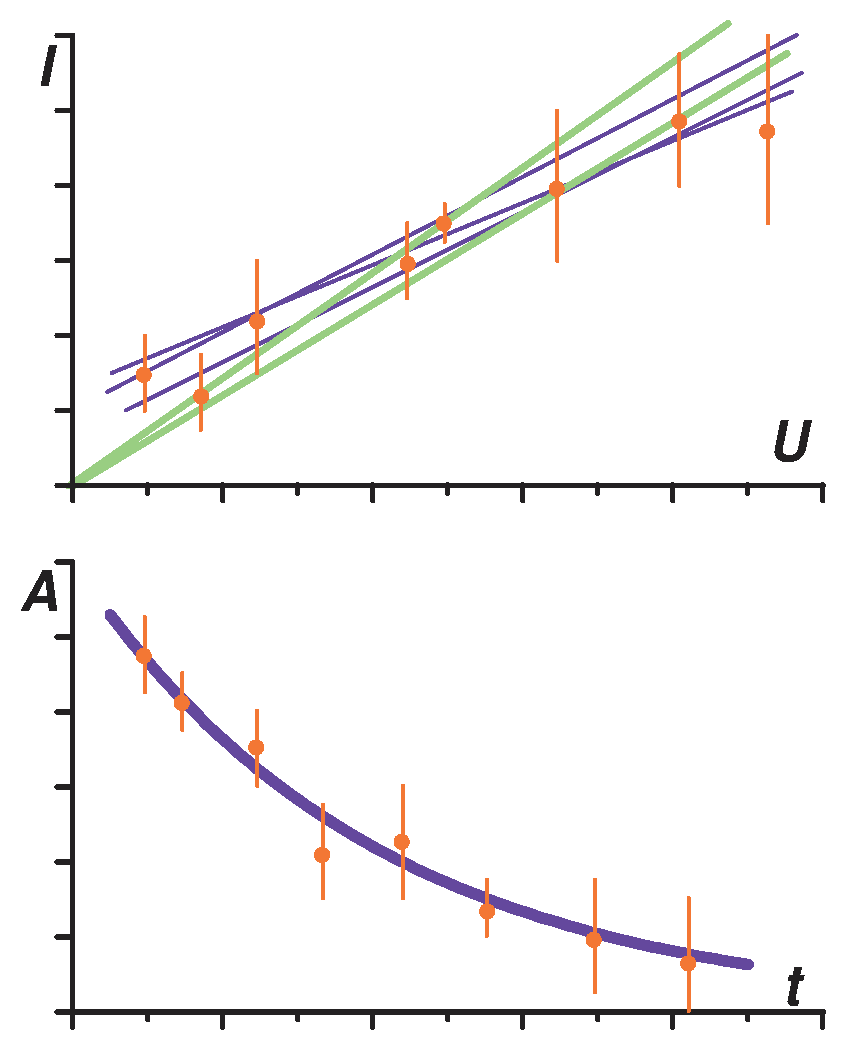
\includegraphics{GP001/GP001F02.eps}}
 \put(25, 165){\makebox(0,0)[l]{\Large\sf Вольт-амперная характеристика}}
 \put(48, 155){\makebox(0,0)[c]{\color{blue}\Huge\bf $I=aU+b$}}
 \put(22, 146){\makebox(0,0)[l]{\color{blue}\Large\bf (какая-то прямая,}}
 \put(22, 141){\makebox(0,0)[l]{\color{blue}\Large\bf надо найти $a$ и $b$)}}
 \put(120, 125){\makebox(0,0)[c]{\color{green}\Huge\bf $I=U/R=k\cdot U$}}
 \put(110, 115){\makebox(0,0)[c]{\color{green}\Large\bf (прямая проходит через О, }}
 \put(110, 109){\makebox(0,0)[c]{\color{green}\Large\bf надо найти наклон $k=1/R$)}}
 \put( 40,  70){\makebox(0,0)[l]{\Large\sf Закон радиоактивного распада}}
 \put(110,  57){\makebox(0,0)[c]{\color{blue}\Huge\bf $A=A_0\cdot e^{-t/\tau}$}}
 \put(105,  47){\makebox(0,0)[c]{\color{blue}\Large\bf (экспонента; надо найти $A_0$ и $\tau$)}}
 \end{picture}
\caption{Примеры фитирования вольт-амперной характеристики (вверху) и данных радиоактивного распада (внизу).}
   \label{fig:fit_fun} % Метка для ссылки на картинку
\end{figure}
 
%\newpage

Итак, надо найти такие значения двух параметров ($A_0$ и $\tau$), чтобы остаточная сумма $\chi^2$ была ми\-ни\-мальной. Условие минимума:

 \begin{displaymath}
\frac{\partial(\chi^2)}{\partial A_0}=0\;\;\;;\;\;\;\;\;\;
\frac{\partial(\chi^2)}{\partial \tau}=0\;\;.
 \end{displaymath}
 \begin{displaymath}
 \left\{
 \begin{array}{cc}
 \sum_i p_i \left[y_i-f(t_i)\right]\frac{\partial f(t_i)}{\partial A_0} &= 0\\[2mm]
 \sum_i p_i \left[y_i-f(t_i)\right]\frac{\partial f(t_i)}{\partial \tau} &= 0
 \end{array}
 \right|\;\;\;\;\;\;\Rightarrow\;\;\;A_0,\;\;\tau
 \end{displaymath}

Если сложный вид $f(x)$ и число параметров $K\gg 1$, то система не решается. Тогда используем \underline{топографический метод}: составляем как бы {\sl карту высот} $\chi^2$ на k-мерной плоскости и ищем на ней низину (Рис.~\ref{fig:2d_fit_surf}).

\begin{figure}[htp] 
 \setlength{\unitlength}{1mm}
 \begin{picture}(165,80)(0,0)
 \put(0, 0){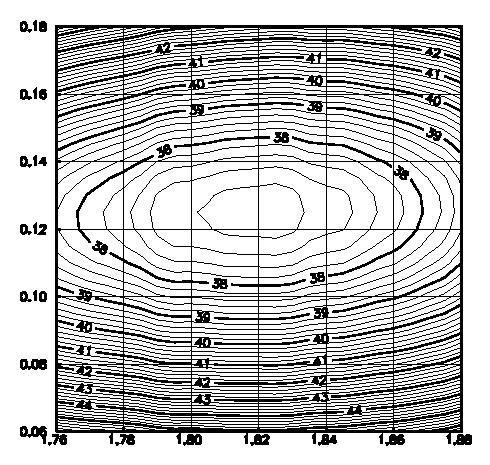
\includegraphics{GP001/GP001F03.eps}}
 \put(85, 0){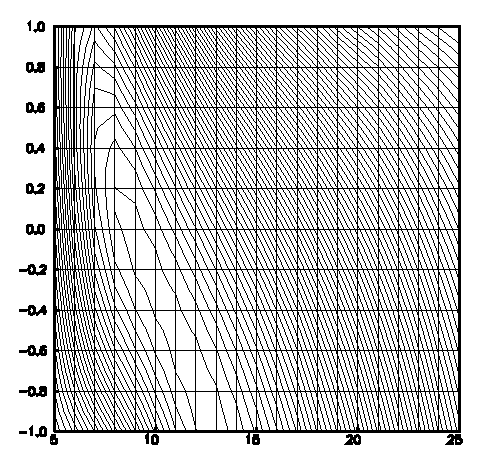
\includegraphics{GP001/GP001F04.eps}}
 {\color{red}
 \put(20,15){\vector(1,4){4}}
 \put(24,31){\vector(1,1){10}}
 \put(34,41){\vector(1,0){6}}
 \color{black}}
 \end{picture}
  \caption{2D-поверхности в фазовом пространстве фитируемых параметров.}
   \label{fig:2d_fit_surf} % Метка для ссылки на картинку
\end{figure}

\underline{Градиентный метод} (то же самое, но низина ищется автоматически). Суть: искомые параметры выбираются наугад (на k-мерной плоскости ставится точка), а затем для этой точки  ищется градиент, то есть, {\color{red}вектор}, показывающий на\-правление максимального изменения $\chi^2$. Находится новая точка, и т. д.  Стандартный программный пакет MINUIT.\\

Свойства  $\chi^2$
\begin{itemize}
\item если "покачать" параметр A на $\pm\Delta A$, то $\chi^2$ увеличится на +1.0
\item нормированное $\chi^2_{\rm norm}=\chi^2/(N-K)$ должно быть $\simeq1$.

Если $\chi^2_{\rm norm}>1$, то неверный вид функции или $\exists$ систематика.

Если $\chi^2_{\rm norm}<1$, то погрешность каждой точки слишком велика.
\end{itemize}
%\newpage

\section{Максимальное Правдоподобие (Maximal Likelyhood)}
%{\color{green}
%{\Huge Максимальное Правдоподобие (Maximal Likelyhood)}\\
%\underline{(Это -- пока вне программы; просто знайте, что %существует и такой метод)}
%}

Если в качестве фитируемых точек используется не измеренная каким-то прибором аналоговая величина $Y_i\pm\Delta Y_i$, а число событий $N_i(X)$ (например, число $\gamma$-квантов, зарегистрированных детектором), то как быть с погрешностью $\Delta N_i$ и весом точек? При больших $N$ погрешность
$\Delta N\simeq\sqrt{N}$, а при малых -- ?...

ML-критерий: надо так подобрать параметры фитирующей функции $f(x)$, чтобы была максимальной вероятность получить в эксперименте именно те точки, которые в нем и получились.

\begin{figure}[ht]
 \setlength{\unitlength}{1mm}
 \begin{picture}(165,90)(0,0)
 \put(0,5){\includegraphics{GP001/GP001F05.eps}}
 \end{picture}
\caption{Распределение пуассона с параметрами задачи в тексте.}
   \label{fig:poisson} % Метка для ссылки на картинку
\end{figure}

\underline{Распределение Пуассона}

Например, мы знаем, что через 1 дм$^2$ пролетает в среднем $\lambda=1.5$ мюона в секунду. Какова вероятность того, что за данную конкретную секунду мы увидим N=1 мюон? N=2 мюона? N=0 мюонов (Рис.~\ref{fig:poisson})? 
\begin{displaymath}
p(N)=\frac{\lambda^N}{N!}e^{-\lambda}
\end{displaymath}


ML-критерий:

\begin{displaymath}
\Phi =\left.\prod_i\frac{\left[f(\overrightarrow{R},x_i)\right]^{N_i}}{N_i!}\cdot e^{-f(\overrightarrow{R},x_i)}\;\right\}\;\;\;\rightarrow\;\max
\end{displaymath}

\section{Литература}
%\newpage
\sf\Large
\renewcommand{\bibname}{}
\phantomsection
\begin{thebibliography}{99}
\bibitem{Фриш}
С.Э.Фриш и А.В.Тиморева, {\bf Курс общей физики}, 3 тома. {\sl\large (ГУ)}\\
{\large
I том: Физические основы механики. Молекулярная физика. Колебания и волны.\\
II том: Электрические и электромагнитные явления.\\
III том: Оптика. Атомная физика.
}
\bibitem{Иродов}
И.Е.Иродов, {\bf Общая физика}. 5 томов {\sl\large (без нумерации. МИФИ.)}\\
{\large
{\sl Механика. Основные законы}.\\
{\sl Физика макросистем. Основные законы}.\\
{\sl Волновые процессы. Основные законы}.\\
{\sl Электромагнетизм. Основные законы}.\\
{\sl Квантовая физика. Основные законы}.
}
\bibitem{Савельев}
И.В.Савельев, {\bf Курс физики}. {\sl\large (3 тома. МИФИ.)}\\
{\large
I том: Механика. Молекулярная физика. \\
II том: Электричество. Колебания и волны. Волновая оптика.\\
III том: Квантовая оптика. Атомная физика. Физика твердого тела. Ядро и частицы.
}
\bibitem{Сивухин}
Д.В.Сивухин, {\bf Курс общей физики}.  {\sl\large (5 томов. МФТИ, Физфак СПбГУ.)}\\
{\large
I том: Механика.\\
II том: Термодинамика и молекулярная физика. \\
III том: Электричество. \\
IV том: Оптика.\\
V том: Атомная и ядерная физика.
}
\bibitem{Калашников}
С.Г.Калашников, {\bf Электричество}.
\bibitem{Тамм}
И.Е.Тамм, {\bf Основы теории электричества}.
\bibitem{Калитеевский}
Н.И.Калитеевский, {\bf Волновая оптика}.
\bibitem{Шпольский}
Э.В.Шпольский, {\bf Атомная физика}.
\bibitem{Борн}
М.Борн, {\bf Атомная физика}.
\bibitem{Мухин}
К.Н.Мухин,  {\bf Экспериментальная ядерная физика}. {\sl\large (2 тома).}
\end{thebibliography}




\topmargin=0cm
\hoffset -30mm
\voffset -12mm
\setlength{\unitlength}{1mm}
\parindent=10mm
\textheight=250mm
\textwidth=185mm
\captionsetup{font={sf,Large}}

\chapter{Классическая механика}
\section{Классическая механика: кинематика + динамика}
\sf\Large
%\centerline{\underline{\Huge\bf Классическая механика}}
%\centerline{кинематика + динамика}
{\sl Г.Галилей (1564-1642)      И.Ньютон (1642-1727)       Л.Эйлер (1707-1783)}

хорошее приближение к действительности (если речь не идет о больших скоростях, больших или малых объектах).

\begin{itemize}
\item Пространство
\item Время
\item Тело
\item Материальная точка
\item Движение
%\item Система координат
\end{itemize}

\section{Кинематика}
%\centerline{\underline{\Huge\bf КИНЕМАТИКА}}

\underline{Прямолинейное равномерное движение}\\

Движение вдоль прямой; равные $\Delta S$ за равные $\Delta t$ (Рис.~\ref{fig:straight_move}).

\begin{figure}[ht]
 \setlength{\unitlength}{1mm}
  \begin{picture}(180,110)(0,0)
  %\put(0,0){\framebox(180,110)[b]{}}
   \put(0,-3){\includegraphics{GP002/GP002F01.eps}}
 \put( 170, 96){\makebox(0,0)[tr]{\parbox{85mm}
     {
     \begin{flushright}
      Пройденный путь: $S=f(t)$\\
      $S_x=f_1(t)$\\
      $S_y=f_2(t)$\\
      $S_z=f_3(t)$
     \end{flushright}
         }}}
  \end{picture}\\[3mm]
  \caption{\sf\Large Движение вдоль прямой.}
   \label{fig:straight_move}
\end{figure}  
%\newpage

{\bf\underline{Скорость равномерного движения} - физ. величина,
прямо пропорциональная пройденному пути
и обратно пропорцио\-нальная затраченному времени.}

\begin{displaymath}
v = \frac{\Delta S}{\Delta t}\;\;\;{\color{blue}(= const)}
\end{displaymath}
 \\[1mm]

{\bf\underline{\color{red}Неавномерное движение:}}

Пример на Рис.~\ref{fig:uneven_move}.

\begin{enumerate}
\item {\underline{\bf OA}} -- торможение
\item {\underline{\bf AB}} -- остановка (состояние покоя)
\item {\underline{\bf BC}} -- ускорение
\item {\underline{\bf CD}} -- равномерное движение
\end{enumerate}

 \begin{figure}[ht]
 \setlength{\unitlength}{1mm}
  \begin{picture}(180,100)(0,0)
  %\put(0,0){\framebox(180,110)[b]{}}
   \put(20,-3){\includegraphics{GP002/GP002F02.eps}}
  \end{picture}\\[3mm]
  \caption{\sf\Large Неравномерное движение.}
   \label{fig:uneven_move}
\end{figure}

{\bf\underline{Средняя скорость:}}\hspace{10mm}
%\begin{displaymath}
$   v_{mean} =  \langle v\rangle  = \overline{v} =  \frac St$\\
%\end{displaymath}

{\bf\underline{Мгновенная скорость в момент $t=\tau$ :}}

\begin{displaymath}
   v(\tau) = \lim_{\Delta t\rightarrow0}\frac{S(\tau+\Delta t)-S(\tau)}{\Delta t} = \frac{dS}{dt}(\tau)= \dot{S}(\tau)
\end{displaymath}
%\newpage

 Путь, пройденный за время от $t_1$ до $t_2$ -- (Рис.~\ref{fig:aver_v_int})?
\begin{displaymath}
S = \sum_i \overline{v_i}\cdot \Delta t_i = \int_{t_1}^{t_2}v(t)dt
\end{displaymath}
 \\[1mm]

\begin{figure}[ht]
 \setlength{\unitlength}{1mm}
  \begin{picture}(180,110)(0,0)
  %\put(0,0){\framebox(180,110)[b]{}}
   \put(0,-3){\includegraphics{GP002/GP002F03.eps}}
  \end{picture}\\[3mm]
\caption{\sf\Large Интегрирование для расчета средней скорости.}
   \label{fig:aver_v_int}
\end{figure}

\underline{\bf Равнопеременное прямолинейное движение}\\[2mm]

Ускорение (положительное или отрицательное):
\begin{displaymath}
v = v_0 + a\cdot t\;\;\;\;\;\;\;\;\;\;\;a = \frac{\Delta v}{\Delta t}
\end{displaymath}

Более точно:
\begin{displaymath}
a = \lim_{\Delta t\rightarrow 0}\left(\frac{\Delta v}{\Delta t}\right)=\frac{dv}{dt}=\dot{v}=\ddot{s}= const
\end{displaymath}

Путь:
\begin{displaymath}
S = \int_{t_1}^{t_2}v(t)dt = v_0\cdot (t_2-t_1) + \frac{a\cdot \left(t_2-t_1\right)^2}2
\end{displaymath}
%\newpage
\underline{\bf Произвольное прямолинейное движение}\\[2mm]

Если задан закон, по которому происходит движение
\begin{displaymath}
 S= f(t)\;\;\;,
\end{displaymath}

то мы всегда сможем найти скорость, ускорение и путь:
\begin{displaymath}
v = \dot{s} = \frac{df}{dt}
\end{displaymath}
\begin{displaymath}
a = \dot{v} = \ddot{s} = \frac{d^2f}{dt^2}
\end{displaymath}
\begin{displaymath}
s = s_2 - s_1 = f(t_2) - f(t_1) \rule[-7mm]{0mm}{12mm}
\end{displaymath}

Поскольку движение имеет {\bf направление}, то s, v и a -- векторы (обозначаются как {\bf s}, {\bf v}, {\bf a} или $\vec{s}$, $\vec{v}$, $\vec{a}$). Все сказанное справедливо (в векторном виде) для криволинейного движения. Положение в пространстве -- радиус-вектор $\vec{r}$ (Рис.~\ref{fig:vec_move}).\\

\begin{figure}[ht]
 \setlength{\unitlength}{1mm}
  \begin{picture}(180,110)(0,0)
  %\put(0,0){\framebox(180,110)[b]{}}
   \put(15,-3){\includegraphics{GP002/GP002F04.eps}}
  \end{picture}\\[3mm]
  \caption{\sf\Large Векторная интерпретация движения.}
   \label{fig:vec_move}
\end{figure}

Составляющие ускорения -- тангенциальное и нормальное (радиальное, центростремительное, Рис.~\ref{fig:a_move}):
 $ \;\;\;\;\vec{a}\;=\;\vec{a_t}\;+\;\vec{a_n}$

\begin{figure}[ht]
\includegraphics[width=0.8\textwidth]{GP002/GP002F05.eps}
% \setlength{\unitlength}{1mm}
%  \begin{picture}(180,45)(0,0)
%  %\put(0,0){\framebox(180,65)[b]{}}
%   \put(15,-3){\includegraphics{GP002/GP002F05.eps}}
%  \end{picture}\\[1mm]
  \caption{\sf\Large Ускорение при движении.}
   \label{fig:a_move}
\end{figure}

Расчеты ускорения через пределы скоростей передвижения расчитываются (Рис.~\ref{fig:a_from_v_move}).

\begin{figure}[ht]
 \setlength{\unitlength}{1mm}
  \begin{picture}(180,80)(0,0)
  %\put(0,0){\framebox(180,70)[b]{}}
   \put(15,-3){\includegraphics{GP002/GP002F06.eps}}
  \end{picture}\\[1mm]
  \caption{\sf\Large Расчет ускорения через пределы векторов скорости.}
   \label{fig:a_from_v_move}
\end{figure}

 \begin{displaymath}
  |dV_t| = |V_2|-|V_1|\;;\;\;\;\;\;  |dV_n| = |V_1|\cdot \varphi
 \end{displaymath}

 \begin{displaymath}
  |a_t| = \lim_{dt\rightarrow0}\frac{|dV_t|}{dt};\;\;\;\;\; \vec{a_t}\parallel\vec{V}
 \end{displaymath}

 \begin{displaymath}
  |a_n| = \lim_{dt\rightarrow0}\frac{|dV_n|}{dt} = \lim_{dt\rightarrow0}\frac{|V_1|\cdot\varphi}{dt}=
  \lim_{dt\rightarrow0}\left(|V_1|\cdot\frac{\varphi}{AB}\cdot\frac{AB}{dt}\right)=
  \frac{|V|^2}R
 \end{displaymath}

 \begin{displaymath}
  \vec{a_n}\parallel \vec{R}\perp \vec{V}
 \end{displaymath}

  \underline{Равномерное} движение по кривой: $\;\;\;|V|$=const, $\;\;\;\; \vec{a}=\vec{a_n}\perp\vec{V}$.

%\newpage
  \underline{\bf Кинематика (абсолютно) твердого тела}\\

  {\bf Поступательное движение --} все точки тела имеют одинаковые скорости и ускорения (Рис.~\ref{fig:trans_move}):

\begin{figure}[ht]
 \setlength{\unitlength}{1mm}
  \begin{picture}(150,60)(0,0)
  %\put(0,0){\framebox(180,80)[b]{}}
   \put(15,0){\includegraphics{GP002/GP002F07.eps}}
  \end{picture}\\[1mm]
  \caption{\sf\Large Поступательное движение твердого тела.}
   \label{fig:trans_move}
\end{figure}

\begin{figure}[ht]
 \setlength{\unitlength}{1mm}
  \begin{picture}(180,92)(0,0)
  %\put(0,0){\framebox(180,100)[b]{}}
   \put(0,0){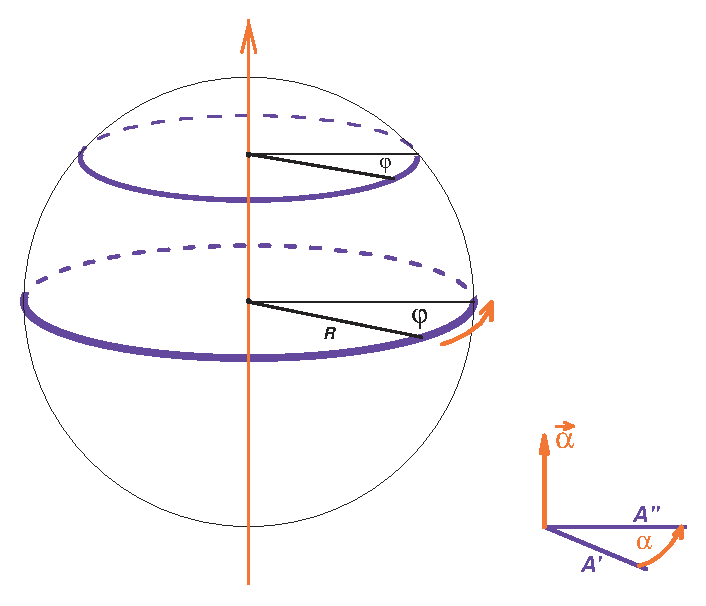
\includegraphics{GP002/GP002F08.eps}}
 \put( 180, 92){\makebox(0,0)[tr]{\parbox{85mm}
     {
     \centerline{\underline{Угловая скорость:}}
      \begin{displaymath}
      \omega=\dot{\varphi}=\frac{d\varphi}{dt}
      \end{displaymath}
     \centerline{\underline{Угловое ускорение:}}
      \begin{displaymath}
      \beta=\dot{\omega}=\ddot{\varphi}=\frac{d\omega}{dt}=\frac{d^2\varphi}{dt^2}
      \end{displaymath}
     }}}
 \put( 175, 0){\makebox(0,0)[br]{\parbox{50mm}
     {
      \centerline{Угол как вектор:}
      \begin{displaymath}
      \vec{\alpha}=\alpha\cdot\frac
          {\left[\vec{A'}\times\vec{A''}\right]}
          {\left|\left[\vec{A'}\times\vec{A''}\right]\right|}
      \end{displaymath}
     }}}
  \end{picture}\\
  \caption{\sf\Large Вращательное движение.}
   \label{fig:rot_move}
\end{figure}

  {\bf Вращение --} все точки тела описывают окружности с центрами на {\sl оси вращения} (Рис.~\ref{fig:rot_move}):

Связь линейной и угловой скорости:

      \begin{displaymath}
      V=\lim_{\Delta t\rightarrow0}\frac{\Delta S}{\Delta t}=\frac{d(R\cdot\varphi)}{dt}=
      \omega R;\;\;\;\;\;\;\;\vec{V}=\left[\vec{\omega}\times\vec{R}\right]
      \end{displaymath}
%\newpage

\underline{\bf Линейные и аксиальные векторы}\\

Линейные (истинные) векторы -- те, что связаны с поступательным движением или направлением в пространстве:

 \begin{displaymath}
 \vec{X}, \vec{Y}, \vec{Z}, \vec{V}, \vec{R}, \vec{a}, \vec{F},
 \end{displaymath}

Аксиальные векторы -- те, что связаны с вращением:

 \begin{displaymath}
 \vec{\varphi}, \vec{\alpha}, \vec{\beta}, \vec{L}, \vec{M}
 \end{displaymath}

Они отличаются своими свойствами симметрии: при зеркальном отра\-жении (то есть, при замене $X \rightarrow -X$) линейные векторы меняют знак, а аксиальные - не меняют (Рис.~\ref{fig:lin_axial_vecs}).

\begin{figure}[htp]
 \setlength{\unitlength}{1mm}
  \begin{picture}(180,150)(0,0)
  %\put(0,0){\framebox(180,150)[b]{}}
   \put(15,0){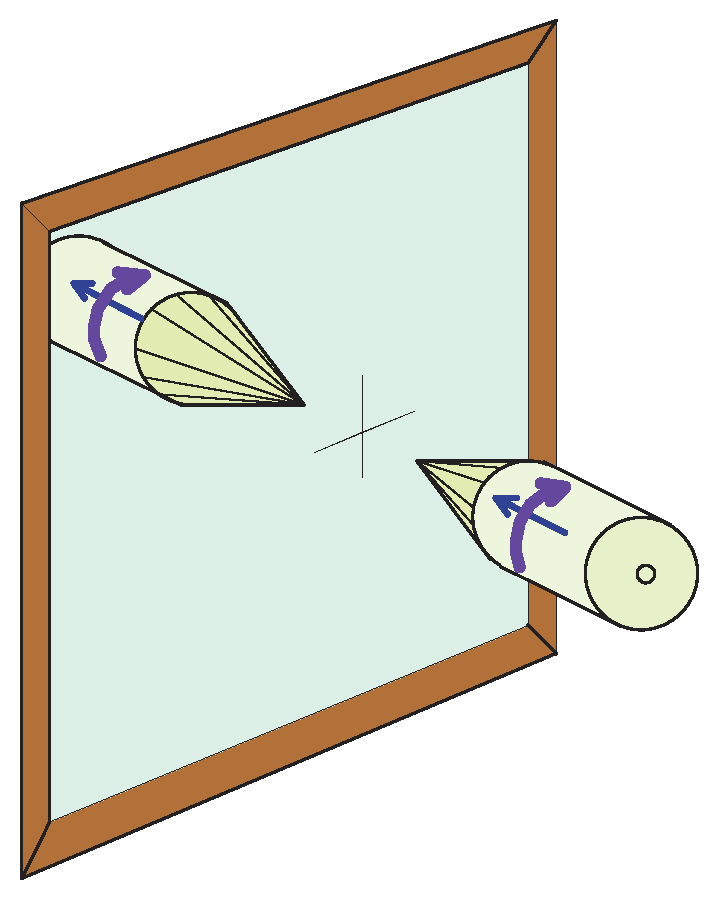
\includegraphics{GP002/GP002F09.eps}}
   \put(48, 105){\makebox(0,0)[c]{\color{blue}\Huge\bf $\vec{\omega}_2$}}
   \put(48, 70){\makebox(0,0)[c]{\color{red}\Huge\bf $\vec{V}_2$}}
   \put(120, 70){\makebox(0,0)[c]{\color{blue}\Huge\bf $\vec{\omega}_1$}}
   \put(120, 35){\makebox(0,0)[c]{\color{red}\Huge\bf $\vec{V}_1$}}
   \put(150,110){\makebox(0,0)[c]{\color{red}\Huge\bf $\vec{V}_2 = -\vec{V}_1$}}
   \put(150, 90){\makebox(0,0)[c]{\color{blue}\Huge\bf $\vec{\omega}_2 = +\vec{\omega}_1$}}
  \end{picture}\\[1mm]
  \caption{\sf\Large Отзеркаливание линейных и аксиальных векторов.}
   \label{fig:lin_axial_vecs}
\end{figure}
  
\newpage
\begin{flushright}
{\color{green}\LARGE\sl ШПАРГАЛКА}
\end{flushright}

\underline{\bf Связь декартовых и сферических координат}

Показана на Рис.~\ref{fig:dec_vs_sphe}.

 \begin{displaymath}
 \left\{\vec{x}, \vec{y}, \vec{z}\right\}
 \;\;\;\leftrightarrow \;\;\;
 \left\{\vec{r}, \vec{\theta}, \vec{\varphi}\right\}
 \end{displaymath}

\begin{figure}[ht]
 \setlength{\unitlength}{1mm}
  \begin{picture}(160,120)(0,0)
  %\put(0,0){\framebox(180,130)[b]{}}
   \put(25,0){\includegraphics{GP002/GP002F10.eps}}
  \end{picture}\\[1mm]
  \caption{\sf\Large Связь декартовых и сферических координат.}
   \label{fig:dec_vs_sphe}
\end{figure}
 
 \begin{displaymath}
 \begin{array}{ccccc}
 0&\leq&r&&\\
 0&\leq&\theta&\leq&\pi\\
 0&\leq&\varphi&\leq&2\pi
 \end{array}
 \end{displaymath}

 \begin{displaymath}
 \left\{
 \begin{array}{ccl}
 x&=&r\sin\theta\cos\varphi\\
 y&=&r\sin\theta\sin\varphi\\
 z&=&r\cos\theta
 \end{array}
 \right\}\;\;\;
 \leftrightarrow\;\;\;
 \left\{
 \begin{array}{ccl}
 r&=&\sqrt{x^2+y^2+z^2}\\
 \theta&=&\arccos\left(z/r\right)\\
 \varphi&=&\arctan\left(y/x\right)
 \end{array}
 \right\}
 \end{displaymath}

 \begin{displaymath}
dx\cdot dy\cdot dz\;\;=\;\;dV\;\;=\;\;r^2\cdot dr\cdot\sin\theta\cdot d\theta\cdot d\varphi
 \end{displaymath}

%\newpage
\begin{flushright}
{\color{green}\LARGE\sl ШПАРГАЛКА}
\end{flushright}
\centerline{\huge\underline{Правила векторной алгебры}}
\begin{itemize}
\item длина вектора (модуль):
 \begin{displaymath}
 |\vec{A}| = \sqrt{A_x^2+A_y^2+A_z^2}
 \end{displaymath}
\item сложение (вычитание):
 \begin{displaymath}
 \vec{C} = \vec{A} \pm \vec{B}\;\;\;\Leftrightarrow\;\;\;
 \left\{\begin{array}{cc}C_x &= A_x\pm B_x\\
                         C_y &= A_y\pm B_y\\
                         C_z &= A_z\pm B_z\end{array}\right.
 \end{displaymath}
\item умножение на число (масштабирование):
 \begin{displaymath}
 \vec{C} = k\cdot\vec{A} \;\;\;\Leftrightarrow\;\;\;
 \left\{\begin{array}{cc}C_x &= k\cdot A_x\\
                         C_y &= k\cdot A_y\\
                         C_z &= k\cdot A_z\end{array}\right.
 \end{displaymath}
\item дифференцирование:
 \begin{displaymath}
 \vec{C} = \frac{\vec{dA}}{dt} \;\;\;\Leftrightarrow\;\;\;
 \left\{\begin{array}{cc}C_x &= {dA_x}/{dt}\\
                         C_y &= {dA_y}/{dt}\\
                         C_z &= {dA_z}/{dt}\end{array}\right.
 \end{displaymath}
\item скалярное перемножение двух векторов:
 \begin{displaymath}
 C = \left(\vec{A},\vec{B}\right) = \vec{A}\cdot\vec{B}\;\;\;\Leftrightarrow\;\;\;
 C = A_x\cdot B_x + A_y\cdot B_y + A_z\cdot B_z =|A|\cdot|B|\cdot \cos\theta
\end{displaymath}
\item векторное перемножение двух векторов:
 \begin{displaymath}
 \vec{C} = \left[\vec{A},\vec{B}\right] = \vec{A}\times\vec{B}\;\;\;\Leftrightarrow\;\;\;
 \left\{\begin{array}{cc}C_x &= A_y\cdot B_z - A_z\cdot B_y\\
                         C_y &= A_z\cdot B_x - A_x\cdot B_z\\
                         C_z &= A_x\cdot B_y - A_y\cdot B_z\end{array}\right.
 \end{displaymath}
 \begin{displaymath}
  |C|=|A|\cdot|B|\cdot\sin\theta;\;\;\;\; \vec{C}\perp\vec{A};\;\;\;\vec{C}\perp\vec{B}
\end{displaymath}
\end{itemize}



\chapter{Динамика}
\sf\Large

%\section{Динамика}
%\centerline{\underline{\Huge\bf ДИНАМИКА}}

\centerline{\sl Изучает взаимодействие тел, приводящее к изменению их движения}
\vspace{2mm}
\section{Первый закон Ньютона (принцип инерции)}
%\underline{\bf Первый закон Ньютона (принцип инерции)}

\begin{center}
\fbox{\parbox{180mm}{\color{blue}\bf Всякое тело сохраняет состояние покоя или равномерного и прямолинейного движения, пока
воздействие со стороны других тел не заставит его изменить это состояние.}}\\[1mm]
(Здесь тело -- как материальная точка, то есть, вращение исключается.)
\end{center}

Наблюдения: 1зН справедлив не для каждой системы отсчета.

\fbox{Инерциальная система} -- та, по отношению к которой 1зН выполняется.

Гелиоцентрическая система. Всякая система, движущаяся относительно нее равномерно и прямолинейно.
\fbox{\color{blue}Инерциальные системы существуют.}\\

\section{Второй закон Ньютона}

%\underline{\bf Второй закон Ньютона}

\begin{center}
\fbox{\parbox{180mm}{\color{blue}\bf Изменение движения пропорционально приложенной силе и происходит в том направлении, в каком действует сила.}}\\[1mm]
\end{center}
Физ. величина СИЛА характеризует воздействие одних тел на другие, в результате которого тела приобретают ускорение.
\begin{displaymath}
 f=k\cdot a\;\;\;\;\;\;\;\;\vec{f}=k\cdot\vec{a}
 \end{displaymath}
Более удобное измерение силы: пружинный динамометр (Рис.~\ref{fig:force_dina}).\\
 
 \begin{figure}[ht]
 \setlength{\unitlength}{1mm}
  \begin{picture}(180,40)(0,0)
   %\put(0,0){\framebox(180,40)[b]{}}
   \put(15,0){\includegraphics{GP003/GP003F01.eps}}
  \end{picture}\\[1mm]
    \caption{Сила и ее измерение пружинным динамометром.}
   \label{fig:force_dina}
\end{figure}
  
Опыт: {\bf разные} тела от {\bf одинаковой} силы получают {\bf разные} ускорения. Это свойство тел -- физ. величина ИНЕРЦИОННАЯ МАССА.\\
Ньютон: МАССА - это мера количества материи в теле {\sl (не совсем верно)}. МАССА - это именно мера инерции.\\
М.В.Ломоносов: масса изолированной системы = const.
\begin{displaymath}
 \vec{a}=k\cdot\vec{f}/m
 \end{displaymath}
%\newpage
Упругие силы, силы тяготения. \underline{\bf Силы трения} -- молекулярное взаимо\-действие между соприкасающимися телами. Трение внешнее (между телом и другими телами; трение покоя) и внутреннее (движение жидкостей и газов).

Сила трения всегда направлена противоположно скорости (Рис.~\ref{fig:fric_force}). Чтобы тело двигалось без ускорения, надо, чтобы внешняя сила уравновешивала силу трения.

\begin{figure}[ht]
 \setlength{\unitlength}{1mm}
  \begin{picture}(180,35)(0,0)
   %\put(0,0){\framebox(180,40)[b]{}}
   \put(10,0){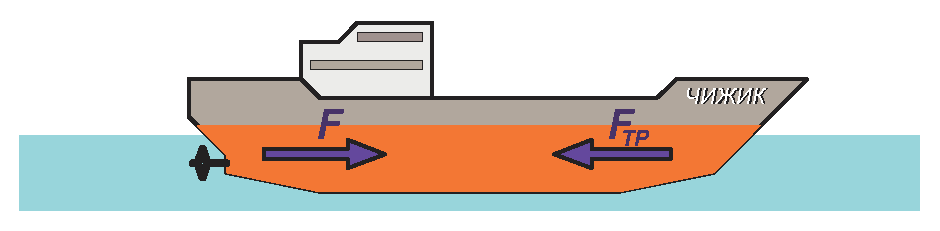
\includegraphics{GP003/GP003F02.eps}}
  \end{picture}\\[1mm]
  \caption{Сила трения всегда направлена против движения.}
   \label{fig:fric_force}
\end{figure}

Парашютист: 60 м/с (открытие парашюта) => 5-6 м/с.

Сила трения скольжения приблизительно пропорциональна сжи\-мающей силе $F_n$ (Рис.~\ref{fig:fric_vec_force}):
\begin{displaymath}
 F_{TP}\simeq\chi\cdot F_n
 \end{displaymath}

\begin{figure}[ht]
 \setlength{\unitlength}{1mm}
  \begin{picture}(180,55)(0,0)
   %\put(0,0){\framebox(180,40)[b]{}}
   \put(45,0){\includegraphics{GP003/GP003F03.eps}}
   \put(0,50){\makebox(0,0)[tl]{\parbox{60mm}{коэффициент трения $\chi$ зависит от состояния поверхностей и от скорости скольжения}}}
  \end{picture}\\[1mm]
\caption{Векторизация силы трения.}
   \label{fig:fric_vec_force}
\end{figure}

Динамика силы трения при начале движения (Рис.~\ref{fig:fric_dyn}).

\begin{figure}[ht]
 \setlength{\unitlength}{1mm}
  \begin{picture}(180,55)(0,0)
   %\put(0,0){\framebox(180,40)[b]{}}
   \put(5,0){\includegraphics{GP003/GP003F04.eps}}
   \put(80,40){\makebox(0,0)[c]{\parbox{85mm}{При V=0 сила трения может быть от 0 до некоего максимума $f$, а при начале движения снижается}}}
   \put(178,30){\makebox(0,0)[tr]{\bf авто: ABS}}
  \end{picture}
    \caption{Динамика силы трения при начале движения.}
   \label{fig:fric_dyn}
\end{figure}

%\newpage
Рассмотрим движение под действием постоянной силы $\vec{f}$ за время $\Delta t$. Используя 2зН, получим:
\begin{displaymath}
  k\cdot\frac{\vec{f}}{m}=\vec{a}=\frac{\vec{v_2}-\vec{v_1}}{\Delta t}
\end{displaymath}
или, домножив на $m$ и $\Delta t$ :
\begin{displaymath}
 m\vec{v_2}-m\vec{v_1} = k\cdot\vec{f}  \Delta t
\end{displaymath}
Величина $m\vec{v}$ имеет большой физический смысл и называется КОЛИЧЕСТ\-ВО ДВИЖЕНИЯ или ИМПУЛЬС (обозначается как $\vec{p}$ -- от англ. {\sl pulse}).
\begin{displaymath}
\vec{p}\equiv m\vec{v}\hspace{40mm} \frac{\vec{dp}}{dt} = k\cdot\vec{f}
\end{displaymath}

Еще одно определение СИЛЫ: Сила -- векторная величина, пропорцио\-нальная вызываемому ею изменению импульса в единицу времени.

Величина $\vec{f}\Delta t$ тоже имеет персональное название -- ИМПУЛЬС СИЛЫ.

Если положить коэф-т $k$ равным 1, то можно установить единицы измерения для $f$.
\begin{itemize}
\item CGS: $[m]$= г, $\;\;[a]$= см/с$^2\;\;\;\;\Rightarrow\;\;\;[f]$= дина = г$\cdot$см/с$^2$
\item SI: $\;\;\;[m]$= кг, $\;[a]$= м/с$^2\;\;\;\;\Rightarrow\;\;\;[f]$= Ньютон = кг$\cdot$м/с$^2 = 10^5$дин
\end{itemize}
\vspace{2mm}

\underline{\bf Механический принцип относительности (Галилей)}

1зН -- частный случай 2зН при $f=0$.

Движение тела относительно двух различных ниерциальных систем отличается лишь на постоянную разность скоростей, а ускорения -- одина\-ковы. $\Rightarrow$ и силы (по 2зН) одинаковы!\\[3mm]
\fbox{\parbox{185mm}{\color{blue}\bf Никакими механическими опытами, производимыми внутри системы, нельзя решить -- находится ли инерциальная система в состоянии покоя или она равномерно и прямолинейно движется. \color{black}\sl Галилей, 1632 г.  }}\\[1mm]

Принцип относительности Эйнштейна: ({\color{blue}механическими})$\rightarrow$({\color{red}любыми: меха\-ническими, электрическими, оптическими, etc.})
%\newpage

\section{Третий закон Ньютона}

%\underline{\bf Третий закон Ньютона} {(\sl Как аукнется -- так и откликнется)}

{\sl Как аукнется -- так и откликнется!}

\begin{center}
\fbox{\parbox{180mm}{\color{blue}\bf Если тело {\bf B} воздействует на тело {\bf A} с силой $\vec{f_1}$, то и тело {\bf A}, в свою очередь, воздействует на тело {\bf B} с силой $\vec{f_2}$, причем $\vec{f_1}=-\vec{f_2}$.} (Рис.~\ref{fig:new_3law})}
\end{center}
%\\[1mm]

\begin{figure}[ht]
 \setlength{\unitlength}{1mm}
  \begin{picture}(180,65)(0,0)
   %\put(0,0){\framebox(180,65)[b]{}}
   \put(0,0){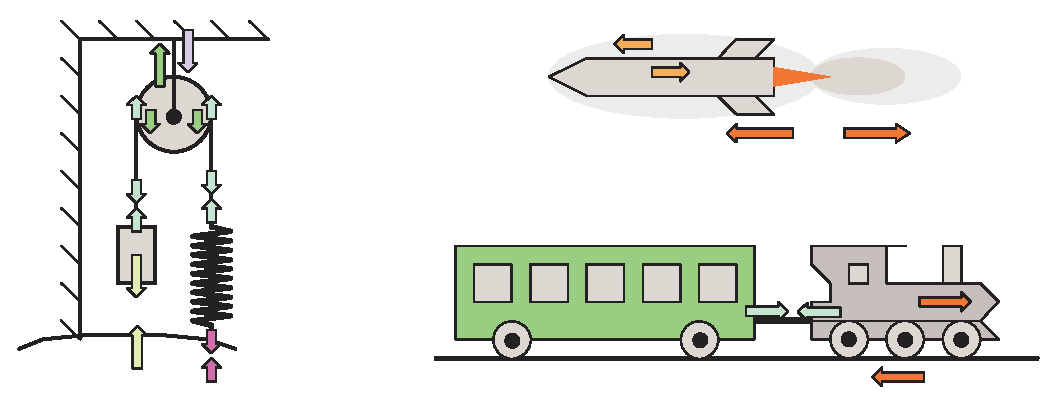
\includegraphics{GP003/GP003F05.eps}}
  \end{picture}\\[1mm]
  \caption{Баланс действия и противодействия (третий закон Ньютона).}
   \label{fig:new_3law}
\end{figure}

Итак, если взаимодействуют 2 тела A и B ;) с массами $m_1$ и $m_2$, то оба приобретают противоположные ускорения:
\begin{displaymath}
\vec{a_1}=\frac{f_1}{m_1},\;\;\;\;\;\;\vec{a_2}=\frac{f_2}{m_2}
\end{displaymath}

Из 3зН следует, что $\vec{f_1}=-\vec{f_2}$, и поэтому
\begin{displaymath}
\vec{a_1}=-\frac{m_2}{m_1}\cdot\vec{a_2}
\end{displaymath}

Изменение количества движения тел A и B:
\begin{displaymath}
\vec{\Delta p_1}=\vec{f_1}\cdot\Delta t\;\;\;\;\;\;\;\vec{\Delta p_2}=
\vec{f_2}\cdot\Delta t=-\vec{\Delta p_1}
\end{displaymath}

\begin{center}
\fbox{\parbox{180mm}{\color{blue}\bf Насколько в результате взаимодействия импульс одного тела увеличился, настолько импульс другого тела уменьшился.}}\\[1mm]
\end{center}

Обобщая на всю систему из N тел, получаем ЗАКОН СОХРАНЕ\-НИЯ КОЛИЧЕСТВА ДВИЖЕНИЯ (ИМПУЛЬСА): $\sum\vec{p} = $const.

\begin{center}
\fbox{\parbox{180mm}{\color{blue}\bf Полный импульс замкнутой системы остается постоянным во все время движения. \color{red}\sl (Не обнаружено нарушений ни в микро-, ни в макро-мире, ни в квантовой, ни в релятивистской механике)}}
\end{center}

%\newpage
Поскольку импульс --- это вектор, то закон сохранения выполняется отдельно для каждой его составляющей (Рис.~\ref{fig:comp_imp_save}):

\begin{figure}[ht]
 \setlength{\unitlength}{1mm}
  \begin{picture}(180,50)(0,0)
   %\put(0,0){\framebox(180,65)[b]{}}
   \put(0,0){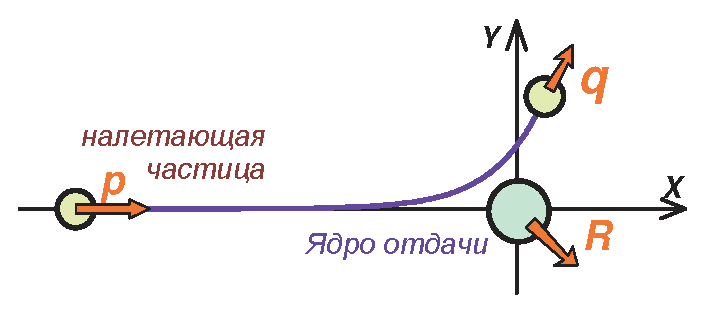
\includegraphics{GP003/GP003F06.eps}}
   \put(180,40){\makebox(0,0)[rt]{\parbox{60mm}{\begin{displaymath}
                                            \left\{ \begin{array}{ccc}
                                            p_x&=&R_x+q_x\\
                                            0&=&R_y+q_y\\
                                            0&=&R_z+q_z
                                                    \end{array}
                                            \right.
                                               \end{displaymath}}}}
  \end{picture}\\[1mm]
  \caption{Сохранение компонент импульса.}
   \label{fig:comp_imp_save}
\end{figure}

\begin{figure}[h]
\centering
\includegraphics[width=0.8\textwidth]{GP003/GP003F07.eps}
% \setlength{\unitlength}{1mm}
%  \begin{picture}(180,80)(0,0)
%   %\put(0,0){\framebox(180,90)[b]{}}
%   \put(0,0){\includegraphics{GP003/GP003F07.eps}}
%  \end{picture}\\
  \caption{Векторный расклад сил при криволинейном движении.}
   \label{fig:vecurve}
\end{figure}

Для изолированной системы из N тел:

\begin{displaymath}
 \vec{P}=\sum_i^N\vec{p_i}=const\;\;\;\Leftrightarrow\;\;\;
 \left\{ \begin{array}{ccccc}
 P_x&=& \sum_{i=1}^N p_{xi}&=&const\\
 P_y&=& \sum_{i=1}^N p_{yi}&=&const\\
 P_z&=& \sum_{i=1}^N p_{zi}&=&const
 \end{array}
 \right.
\end{displaymath}
\hspace{3mm}

\underline{\bf Силы при криволинейном движении}

Как и ускорение, сила имеет 2 компонента (Рис.~\ref{fig:vecurve}):

\begin{enumerate}
\item тенгенциальная сила ($\vec{f_t}\parallel\vec{v}$ -- разгоняет или тормозит)
\item центростремительная сила ($\vec{f_n}\perp\vec{v}$ -- заставляет менять направление)
\end{enumerate}

\begin{displaymath} \vec{f}=\vec{f_t}+\vec{F_n};\;\;\;\;\;\;\;|f|=\sqrt{f_t^2+f_n^2};\;\;\;\;\;\;\;\;
 |f_n|=ma_n=m \frac{v^2}{R}
\end{displaymath}

%\newpage
\noindent
Равномерное движение по кривой: $f_t=0$. Вся сила -- центростремительная.\\[4mm]
Равномерное движение по окружности: $R=$const., $v=\omega R$
\begin{displaymath}
 f_n=m \frac{v^2}{R}=m\omega^2R=4\pi^2m\frac{R}{T^2}
\end{displaymath}

\underline{Центростремительная} сила приложена к телу, а равная ей (но противопо\-ложная по направлению) \underline{центробежная} -- к связям. В реальных задачах иногда требуется компенсация (Рис.~\ref{fig:vagon_balance}).
\\

\begin{figure}[ht]
 \setlength{\unitlength}{1mm}
  \begin{picture}(180,60)(0,0)
   %\put(0,0){\framebox(180,65)[b]{}}
   \put(85,0){\includegraphics{GP003/GP003F08.eps}}
   \put(0,0){\makebox(0,0)[bl]{\parbox{130mm}{\sf\Large
    Неподвижный вагон, кроме нормальной к рельсам силы $f_0$, оказывает на них боковое давление с силой $f_s=P\;{\rm tg}\alpha$. Надо, чтобы при движении центробежная сила ее скомпенсировала:
   \begin{displaymath}
   P\cdot tg\alpha = mg\cdot tg\alpha = \frac{mv^2}{R}\;\;\;\;\Rightarrow\;\;\;
   tg\alpha = \frac{mv^2}{Rg}
   \end{displaymath}}}}
  \end{picture}\\[1mm]
  \caption{Наклон вагона для компенсации бокового давления при движении по окружности.}
   \label{fig:vagon_balance}
\end{figure}

\newpage
\underline{\bf Ускоренные системы}
\\

В ускоренных системах возникают силы, действующие на компоненты системы (Рис.~\ref{fig:a_system}). 

\begin{figure}[ht]
 \setlength{\unitlength}{1mm}
  \begin{picture}(180,40)(0,0)
   %\put(0,0){\framebox(180,65)[b]{}}
   \put(0,0){\includegraphics{GP003/GP003F09.eps}}
   \put(190,0){\makebox(0,0)[br]{\parbox{90mm}{\sf\Large
   В Лаб.системе: вагон ускоряется, шар отстает.\\
   В системе вагона: шар покатился назад с ускорением $-a$, как если бы появилась сила
   $\vec{f}=-m\vec{a}$
   }}}
  \end{picture}\\[1mm]
  \caption{Силы в ускоренной системе.}
   \label{fig:a_system}
\end{figure}

Фиктивная сила, которую приходится вводить в ускоренной системе отсчета, чтобы в ней выполнялся 2 закон Ньютона -- \underline{инерционная сила} или \underline{сила инерции} (Рис.~\ref{fig:iner_a_sys}).
\\

\begin{figure}[ht]
 \setlength{\unitlength}{1mm}
  \begin{picture}(180,90)(0,0)
   %\put(0,0){\framebox(180,80)[b]{}}
   \put(0,0){\includegraphics{GP003/GP003F10.eps}}
   \put(190,0){\makebox(0,0)[br]{\parbox{130mm}{\sf\large
   \begin{enumerate}
   \item{\bf $\vec{a}=0$ (Лифт стоит на месте или движется равномерно.)}
        Гиря давит на весы своим весом $\vec{P}=m\vec{g}$. Весы давят на гирю с такой же силой и уравновешивают ее вес. (В обеих {\bf инерциальных} системах координат)
   \item{\bf $\vec{a}>0$ (Лифт ускоряется вверх.)}
    \begin{itemize}
    \item В Лаб.системе: Чтобы гиря тоже начала ускоряться вместе с лифтом, весы давят на нее снизу с дополнительной силой $\vec{f\prime}=m\vec{a}$. По 3зН гиря давит на весы с такой же силой.
    \item В системе лифта: появилась сила инерции $\vec{f\prime\prime}=-m\vec{a}$, которая добавилась к весу гири.
    \end{itemize}
   \end{enumerate}
   }}}
  \end{picture}\\[1mm]
    \caption{Силы инерции в ускоренной системе.}
   \label{fig:iner_a_sys}
\end{figure}

  ОТО Эйнштейна: Вселенная относительно системы лифта дернулась вниз с ускорением $-\vec{a}$ и создала дополнительное гравитационное поле, направ\-ленное туда же:
   $g\;\;\;\rightarrow\;\;\;g\prime=(g+a)$.\\[1mm]

%\newpage
\underline{\bf Вращающиеся системы}

Баланс сил во вращающейся системе показан на Рис.~\ref{fig:rot_sys_balance}.

\begin{figure}[ht]
 \setlength{\unitlength}{1mm}
  \begin{picture}(180,100)(0,0)
   %\put(0,0){\framebox(180,65)[b]{}}
   \put(0,0){\includegraphics{GP003/GP003F11.eps}}
   \put(190,0){\makebox(0,0)[br]{\parbox{100mm}{\sf\Large
   В инерциальной гелиоцентрической системе: чтобы тело А на широте $\varphi$ вращалось вместе с Землей вокруг ее оси, надо, чтобы часть его веса $P_0$ играла роль центростремительной силы ${\color{green}f}=m\omega^2r=m\omega^2R\cos\varphi$.\\
   В системе, связанной с Землей: 1) направленный к центру Земли вес $P_0$  и 2) {\sl инерционная центробежная сила} ${\color{red}f\prime}=m\omega^2r$, направленная от оси. Их сумма - кажущийся вес ${\color{magenta}P}$.\\
   Масштаб: $f/P_0=\omega^2R\cos\varphi/g\simeq\cos\varphi/289$
   }}}
  \end{picture}\\[1mm]
  \caption{Баланс сил во вращающейся системе.}
   \label{fig:rot_sys_balance}
\end{figure}
  
На экваторе ($\varphi=0$): $f/P_0$ -- максимально; \hfill{} $f_{\max}/P_0=\omega^2R/g=v^2/gR$\\
Обращается в 1 при $v=\sqrt{gR}\simeq7.9$ км/с

\newpage

\centerline{\underline{\bf Сила Кориолиса}}

% \begin{figure}[ht]
 \setlength{\unitlength}{1mm}
  \begin{picture}(180,240)(0,0)
   %\put(-5,-10){\framebox(180,240)[b]{}}
   \put(0,-10){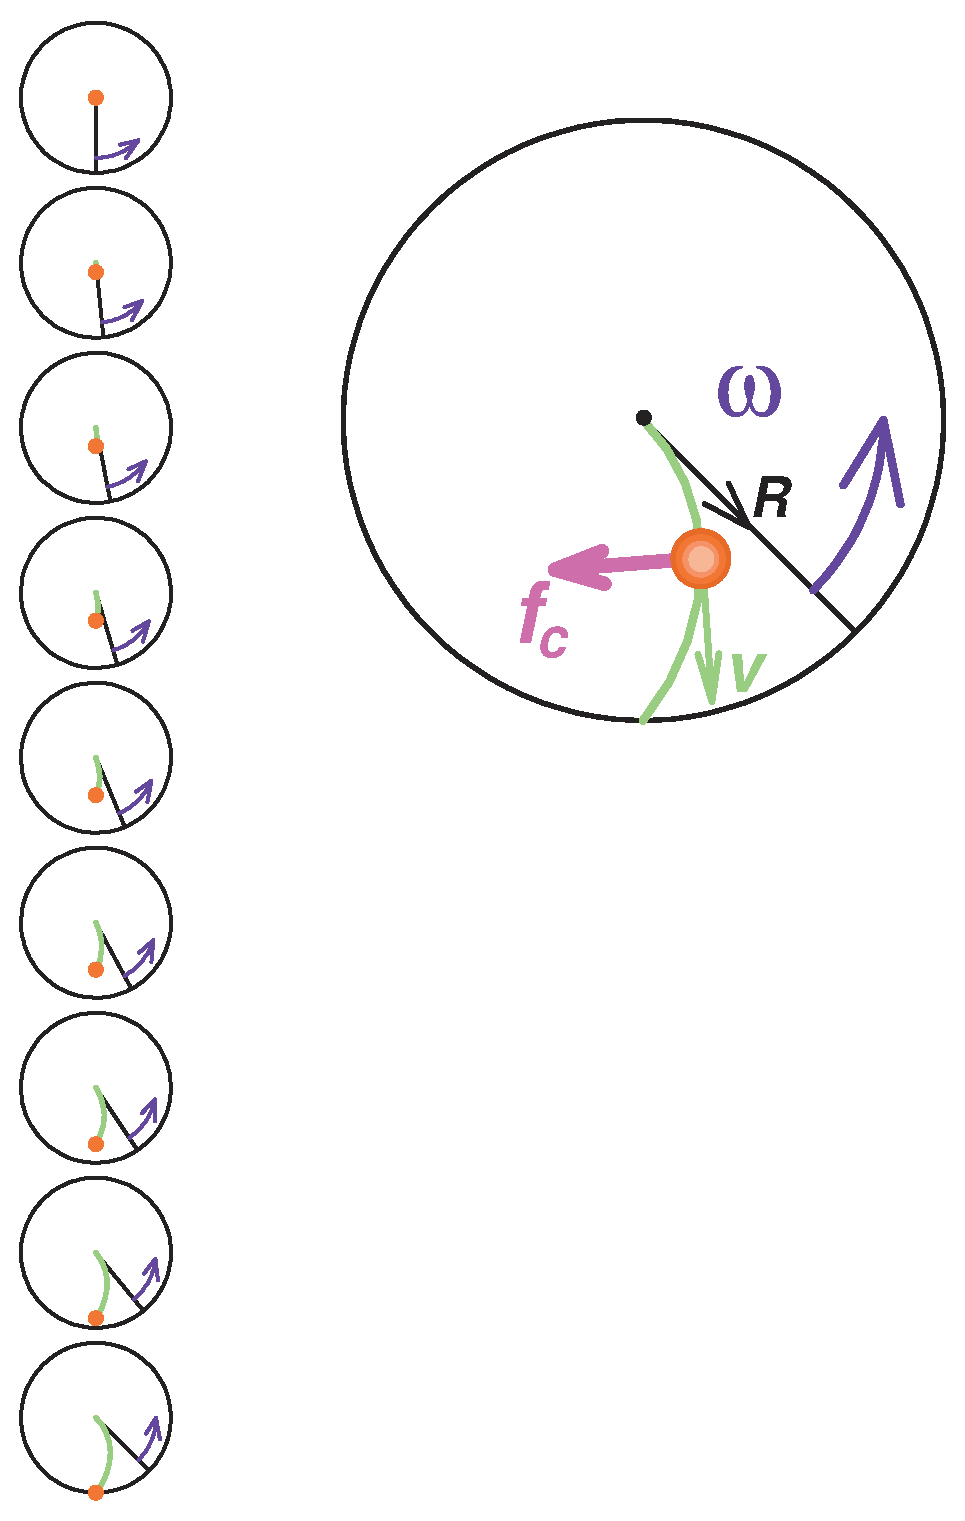
\includegraphics{GP003/GP003F12.eps}}
   \put(100,231){\makebox(0,0)[c]{Шарик катится по вращающемуся диску:}}
   \put(35,120){\makebox(0,0)[tl]{\parbox{40mm}{В лабораторной (инерциальной!) системе -- O.K. }}}
   \put(180,115){\makebox(0,0)[tr]{\parbox{80mm}{В системе диска шарик сносит вправо, как если бы на него действовала сила $\vec{f_c}\perp\vec{v}$}}}
   \put(180,0){\makebox(0,0)[br]{\parbox{150mm}{Мы живем в такой вращающейся системе. Чтобы корректно объяснить все явления, у нас $\exists$ два выхода:
   \begin{enumerate}
   \item Каждый раз переделывать все формулы, учитывая вращение системы координат
   \item Ввести фиктивную (как и силу инерции) Кориолисову силу $\vec{f_c}$, которая $\perp$ скорости $\vec{v}$ и оси вращения $\vec{\omega}$.
   \end{enumerate}
   \begin{displaymath}
    \vec{f_c}=2m\left[\vec{v}\times\vec{\omega}\right]
   \end{displaymath}
   }}}
  \end{picture}\\[1mm]
%  \caption{.}
%   \label{fig:}
%\end{figure}
  
\underline{\bf Вывод формулы для силы Кориолиса} \hfill{ } {\color{green}\sl (факультативно)}

Пусть тело движется со скоростью $\vec{v}$ и ускорением $\vec{a}$ в неинерциальной системе координат, которая вращается с угловой скоростью $\vec{\omega}$ и угловым ускорением $\vec{\beta}$. Если радиус вращения тела равен $\vec{R}$,
то линейная скорость $\vec{v\prime}$ во внешней \underline{инерциальной} системе равна:
   \begin{displaymath}
    \vec{v\prime}= \vec{v}+\left[\vec{\omega}\times\vec{R}\right]
   \end{displaymath}
 Ускорение $\vec{a\prime}$ этой инерциальной системе равно:
   \begin{displaymath}
   \vec{a\prime}= \frac{d}{dt}\left(\vec{v\prime}\right) =
   \frac{d}{dt}\left(\vec{v}\right) +
   \frac{d}{dt}\left[\vec{\omega}\times\vec{R}\right]=
   \frac{d}{dt}\left(\vec{v}\right) +
   \left[\frac{d}{dt}\left(\vec{\omega}\right)\times\vec{R}\right] +
   \left[\vec{\omega}\times\frac{d}{dt}\left(\vec{R}\right)\right]\;.
   \end{displaymath}
 Учитывая, что
   \begin{displaymath}
   \frac{d}{dt}\left(\vec{v}\right) = \vec{a}+\left[\vec{\omega}\times\vec{v}\right],
   \end{displaymath}
 а скорость изменения радиуса
   \begin{displaymath}
   \frac{d}{dt}\left(\vec{R}\right) = \vec{v}+\left[\vec{\omega}\times\vec{R}\right],
   \end{displaymath}
получим:
   \begin{displaymath}
   \vec{a\prime}=
   \vec{a}+
   \left[\vec{\omega}\times\vec{v}\right]+
   \left[\vec{\beta}\times\vec{R}\right]+
   \left[\vec{\omega}\times\vec{v}\right]+
   \left[\vec{\omega}\times\left[\vec{\omega}\times\vec{R}\right]\right].
      \end{displaymath}
Далее воспользуемся свойством тройного векторного произведения
   \begin{displaymath}
\left[\vec{A}\times\vec{B}\times\vec{C}\right] =
\vec{B}\cdot\left(\vec{A}\cdot\vec{C}\right) -
\vec{C}\cdot\left(\vec{A}\cdot\vec{B}\right),
      \end{displaymath}
а также тем фактом, что векторы $\vec{\omega}$ и $\vec{R}$ взаимно перпендикулярны, и потому их скалярное произведение равно нулю:
   \begin{displaymath}
   \left[\vec{\omega}\times\left[\vec{\omega}\times\vec{R}\right]\right]=
   \vec{\omega}\cdot\left(\vec{\omega}\cdot\vec{R}\right)-
   \vec{R}\cdot\left(\vec{\omega}\cdot\vec{\omega}\right)=
   -\vec{R}\cdot\omega^2.
   \end{displaymath}
Итак, получаем, что ускорение тела относительно инерциальной системы, в которой просто обязаны соблюдаться все законы Ньютона, равно:
   \begin{displaymath}
   \vec{a\prime}=
   \vec{a}+
   \left[\vec{\beta}\times\vec{R}\right]-
   2\left[\vec{v}\times\vec{\omega}\right]-
   \omega^2\vec{R}.
   \end{displaymath}
 Если почленно умножить все это на массу $m$, то в последнем слагаемом узнаем центростремительную силу, которая должна уравновесить силу инерции, направленную по радиусу, а в предпоследнем - силу, которая должна скомпенсировать силу Кориолиса (если мы не хотим, чтобы тело отклонилось от своего заданного движения в неинерциальной системе).



\chapter{Работа и энергия}
\input{GP004/GP004_section.tex}

\chapter{Движение твердого тела}
\input{GP005/GP005_section.tex}

\chapter{Движение жидкости}
\input{GP006/GP006_section.tex}

\chapter{Элементы СТО}
\input{GP007/GP007_section.tex}

\chapter{Молекулярная физика}
\input{GP008/GP008_section.tex}

\chapter{Распределение Максвелла}
\input{GP009/GP009_section.tex}

\chapter{Микро- и макро-явления в газах}
\input{GP010/GP010_section.tex}

\chapter{Реальные газы}
\sf\Large

%\centerline{\LARGE\bf РЕАЛЬНЫЕ ГАЗЫ}
До сих пор мы говорили об {\bf идеальном газе}: молекулы -- это твердые шарики, соударяющиеся упруго. Размерами пренебрегаем. Взаимодействие -- только в момент удара.

Однако, мы знаем, что при больших давлениях законы Бойля-Мариотта и Гей-Люссака не работают. Причины очевидны:
\begin{enumerate}
\item Молекулы -- не точечные; в формулах надо учитывать их размеры, которые при большом давлении занимают существенную долю объема.
\item Молекулы -- не твердые шарики; силы взаимодействия между ними имеют сложный характер.
\end{enumerate}
 \begin{picture}(185,35)(0,0)
 %\put(0,0){\framebox(185,35)[b]{}}
 \put(10,0){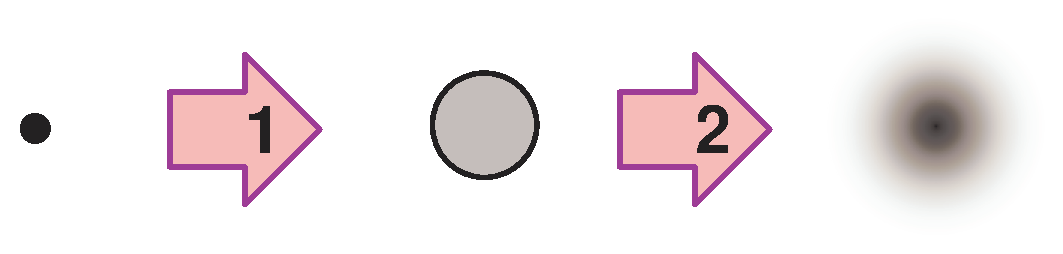
\includegraphics{GP011/GP011F01.eps}}
 %\put(0,0){\makebox(0,0)[tl]{\parbox{125mm}{}}}
 \end{picture}\\

 Ван-дер-Ваальс (Johannes Diderik van der Waals, 1837 - 1923, Amsterdam) все это учел.
Для идеального газа было
\begin{displaymath}
pV_0=RT
\end{displaymath}
1) Если считать суммарный объем всех молекул равным $b$, то получится, что эффективный простор, в котором могут метаться молекулы, меньше реального объема газа на эту величину, и уравнение преображается:
\begin{displaymath}
p(V_0-b)=RT
\end{displaymath}
2) На большом расстоянии молекулы слегка притягиваются друг к другу, и газ немного сжимается, как если бы давление было повыше -- не $p$, а $p+p_i$, где $p_i$ -- некое ``внутреннее'' давление. Итого, имеем
\begin{displaymath}
(p+p_i)(V_0-b)=RT
\end{displaymath}
Осталось как-то определить величину этих поправок. Сначала определимся с величиной $b$. Пусть в объеме есть только 2 молекулы с радиусом $r$ и объемом $v=\frac43\pi r^3$. Какой объем недоступен для их движения? Ответ: центры молекул не могут сблизиться меньше чем на $2r$. То есть, на двоих недоступен объем $\frac43\pi (2r)^3=8v$, а на одну молекулу -- $4v$. Итак, поправка $b$ примерно равна учетверенному суммарному объему всех молекул.

Если с поправкой $b$ все ясно, то с ``внутренним давлением'' все сложнее.
 
 \begin{picture}(185,30)(0,0)
 %\put(0,0){\framebox(185,30)[b]{}}
 \put(145,0){\includegraphics{GP011/GP011F02.eps}}
 \put(0,28){\makebox(0,0)[tl]{\parbox{140mm}{
В целом, молекулы нейтральны и кулоновски притягиваться не могут. Но зато могут поляризоваться! Причина при\-тя\-же\-ния -- в поляризации.
Действительно: при дан\-ном расположении диполей, расстояние между }}}
 \end{picture}\\
разноименными зарядами меньше, чем между одноименными ($R_A<R_r$), и поскольку силы как притяжения, так и отталкивания, $\sim 1/R^2$, то на небольших расстояниях притяжение пересиливает. Если считать, что {\bf каж\-дый} из N диполей, находящихся в некотором рассматриваемом объеме, взаимодействует с {\bf каждым} из остальных N--1, то количество притягива\-ю\-щих связей
=N(N--1). При большом N это превращается в $\simeq$N$^2$. Таким образом, вторая поправка, связанная с притяжением молекул, должна быть $\sim$ квадрату числа молекул в единице объема $\sim n_0^2$ или обратно пропорциональна квадрату молярного объема $\sim1/V_0^2$.

Итак, уравнение Ван-дер-Ваальса:
\begin{equation}
\left(p+\frac{a}{V_0^2}\right)\left(V_0-b\right)=RT
\end{equation}
Если у нас не 1 моль газа, а, например, некая масса $m$, то занимаемый газом объем $V$ будет в $m/\mu$ раз больше: $V=V_0\cdot m/\mu$. Выразив отсюда $V_0$ через $V$, подставим его в уравнение:
\begin{equation}
\left(p+\frac{m^2}{\mu^2}\frac{a}{V^2}\right)\left(V-\frac{m}{\mu}b\right)=\frac{m}{\mu}RT
\end{equation}
 \begin{picture}(185,42)(0,0)
 %\put(0,0){\framebox(185,40)[b]{}}
 \put(55,0){\includegraphics{GP011/GP011F04.eps}}
 \put(0,38){\makebox(0,0)[tl]{\parbox{50mm}{
Это выполняется уже гораздо лучше, чем уравнение для идеальных газов, но все же не точно.
 }}}
 \end{picture}\\
 \begin{picture}(185,75)(0,0)
 %\put(0,0){\framebox(185,75)[b]{}}
 \put(15,0){\includegraphics{GP011/GP011F03.eps}}
 \put(0,38){\makebox(0,0)[tl]{\parbox{50mm}{
 }}}
 \end{picture}\\
Силы между молекулами: отталкивание ($f_{\rm repulsion}$) и притяжение ($f_{\rm attraction}$). Потенциальная энергия $E_r>0$ и $E_a<0$. Притяжение с расстоянием убывает медленнее, зато отталкивание при $r\rightarrow0$ растет круче.

Объяснение: как уже говорилось, молекулы издали слегка притяги\-ва\-ют\-ся друг к другу из-за поляризации. Вблизи же, когда их электронные оболочки соприко\-с\-ну\-лись, начинается резкое кулоновское отталкивание ядер, т.к. оболочки их (ядра) больше не экранируют.

В итоге имеем характерную кривую с минимумом при $r=r_0$. Если бы у молекул не было кинетической энергии, то они бы расположились на $r_0$ друг от друга и так в этих потенциальных ямах и сидели бы. На самом же деле, имея какую-то $E_k>0$, соответствующую данной температуре, они сближаются, немного даже разгоняясь из-за притяжения (пунктир обозначает уровень ПОЛНОЙ энергии $E=E_p+E_k$). При $r<r_0$ молекулы ``проскакивают'' точку равновесия, начинают тормозиться и совсем оста\-на\-в\-ли\-ваются при $r=s$ (это максимально возможное сближение), а затем снова разлетаются.\\
 \begin{picture}(185,45)(0,0)
 %\put(0,0){\framebox(185,45)[b]{}}
 \put(15,20){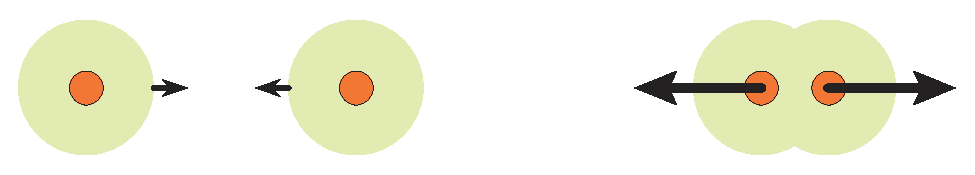
\includegraphics{GP011/GP011F05.eps}}
 \put(50,15){\makebox(0,0)[t]{\parbox{55mm}{
 Слабое притяжение нейтральных молекул
 }}}
 \put(145,15){\makebox(0,0)[t]{\parbox{58mm}{
 Сильное отталкивание положительных ядер
 }}}
 \end{picture}\\
 \begin{picture}(190,110)(0,0)
 %\put(0,0){\framebox(190,110)[b]{}}
 \put(0,0){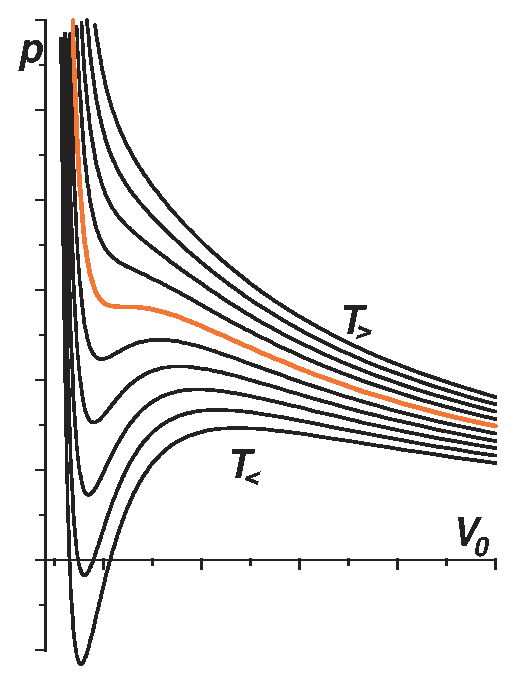
\includegraphics{GP011/GP011F06.eps}}
 \put(50,110){\makebox(0,0)[tl]{\parbox{140mm}{
 Уравнение состояния газа Ван-дер-Ваальса
 \begin{displaymath}
\left(p+\frac{a}{V_0^2}\right)\left(V_0-b\right)=RT
\end{displaymath}
  }}}
 \put(90,83){\makebox(0,0)[tl]{\parbox{100mm}{
 -- это уравнение 3 степени относительно $V_0$ при постоянных $p$ и $T$. Оно должно иметь 3 решения: при $T<T_k$ -- все вещественные, при $T>T_k$ -- одно вещественное и два комплексных.\\

 При большой $T$ кривая $p(V_0)$ ведет себя как изотерма для идеального газа, соответствующая закону Бойля-Мариотта $\left( pV_0={\rm const.}\right)$, а при малой...
  }}}
 \end{picture}\\
 \begin{picture}(190,110)(0,0)
 %\put(0,0){\framebox(190,110)[b]{}}
 \put(0,0){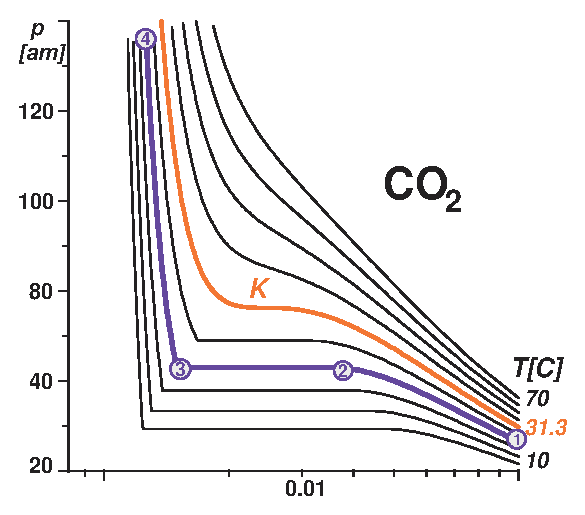
\includegraphics{GP011/GP011F07.eps}}
 \put(135,40){\includegraphics{GP011/GP011F08.eps}}
 \put(20,110){\makebox(0,0)[tl]{\parbox{130mm}{
Будем сжимать газ CO$_2$, поддерживая его температуру постоянной, и записывать величину давления при разном объеме.
  }}}
 \put(190,0){\makebox(0,0)[br]{\parbox{85mm}{
участок (1---2): давление растет.\\
участок (2---3): газ сжижается, давление остается постоянным.\\
участок (3---4): сжатие жидкости.
  }}}
 \end{picture}\\

 Давление, при котором происходит сжижение, -- {\bf упругость на\-сы\-щен\-ных паров при данной температуре}.
 
 %\newpage
 \noindent
 \begin{picture}(190,105)(0,0)
 %\put(0,0){\framebox(190,105)[b]{}}
 \put(0,0){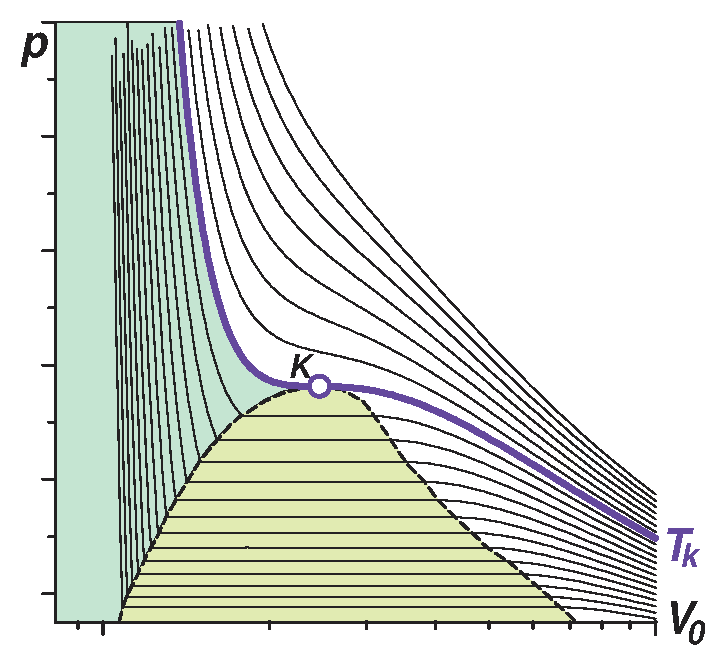
\includegraphics{GP011/GP011F09.eps}}
 \put(60,106){\makebox(0,0)[tl]{\parbox{130mm}{
 Если температура выше критической, то сжижение невозможно. Изотерма, которая отделяет семейство изотерм с провалом от семейства изотерм без провала, -- {\bf критическая изотерма}.
  }}}
 \put(120,75){\makebox(0,0)[tl]{\parbox{70mm}{
 При температуре ниже кри\-тической вещество мо\-жет существовать либо как газ, либо как жидкость, либо как и жид\-кость и на\-сы\-щен\-ный пар од\-но\-вре\-мен\-но (в зависимости от давления). Для воды, e.g., $T_k=374^\circ$C.
 Упругость насыщенного па\-ра $\leq p_k$ (критическое дав-
  }}}
 \end{picture}\\
ление). Объем жидкости $\leq V_k$ (критический объем). В критической точке пропадает всякое различие между жидкостью и газом.

При $p<p_0$ (давления насыщенного пара) можно получить жидкость в ($\bullet$){\bf A} без ее перехода в газ (растянутая жидкость). Аналогично, при $p>p_0$ можно получить газ в ($\bullet$){\bf B} без его конденсации (пересыщенный пар).\\
 \begin{picture}(190,100)(0,0)
 %\put(0,0){\framebox(190,100)[b]{}}
 \put(0,0){\includegraphics{GP011/GP011F10.eps}}
 \put(110,98){\makebox(0,0)[tl]{\parbox{80mm}{
 Оба эти состояния очень не\-устойчивы. При появлении малейшей ``провокации'' рас\-тя\-ну\-тая жидкость закипает, а пере\-сы\-щен\-ный пар кон\-ден\-си\-ру\-ет\-ся (вспомните иммерсион\-ный след за самолетом).
  }}}
 \put(125,44){\makebox(0,0)[tl]{\parbox{65mm}{
  Первое явление использу\-ет\-ся для регистрации субатомных частиц в пузырьковой камере, а второе -- в камере Вильсона.
  }}}
 \end{picture}\\
\underline{\bf Внутренняя энергия реального газа.}

Как ранее говорилось, для \underline{идеального газа} внутренняя энергия $U$ -- это кинетическая энергия движения молекул:
\begin{displaymath}
U = E_k=\sum\overline{w}_k = C_V\;T
\end{displaymath}
Она не зависит ни от давления, ни от объема, а только от температуры и вида молекул.

В \underline{реальном} же газе $\exists$ силы между молекулами (и притяжение, и отталкивание) $\Rightarrow$ кроме кинетической $\exists$ еще и потенциальная энергия
\begin{displaymath}
U = E_k + E_p
\end{displaymath}
 \begin{picture}(185,80)(0,0)
 %\put(0,0){\framebox(185,75)[b]{}}
 \put(15,0){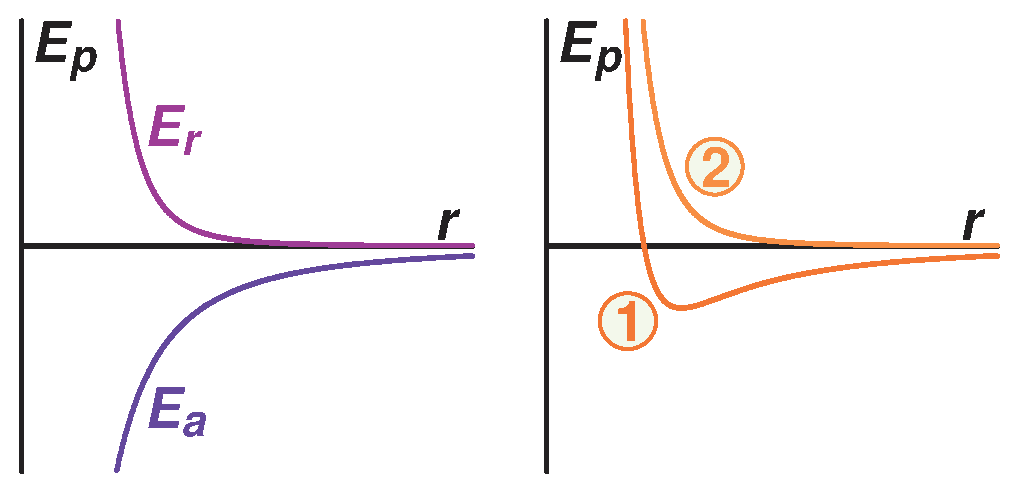
\includegraphics{GP011/GP011F11.eps}}
 \put(0,38){\makebox(0,0)[tl]{\parbox{50mm}{
 }}}
 \end{picture}\\
Как мы видели, $E_p$ зависит от расстояния между молекулами $\Rightarrow$ зависит от объема $V$.

Если объем увеличить (без совершения внешней работы), то притяже\-ние ослабнет, потенциаль\-ная энергия слегка возрастет, а кинетической придется уменьшится (чтобы полная энергия не изменилась). Иначе говоря, при удалении молекул друг от друга притяжение их слегка притормаживает. В итоге, скорость молекул упадет $\Rightarrow$ температура тоже упадет!

Btw, еще не факт, кто ``побеждает'' на больших расстояниях -- притяже\-ние (результирующая кривая 1) или отталкивание (кривая 2)... Если оттал\-ки\-ва\-ние -- то при расширении газа скорость (и температура) только увели\-чит\-ся.

 Джеймс Джоуль пытался в конце IXX века это обнаружить. Удалось позднее, когда они вместе с Вильямом Томсоном заменили кран на пористую пробку ({\bf дросселирование})\\ \begin{picture}(185,110)(0,0)
 %\put(0,0){\framebox(185,75)[b]{}}
 \put(10,0){\includegraphics{GP011/GP011F12.eps}}
 \put(0,38){\makebox(0,0)[tl]{\parbox{50mm}{
 }}}
 \end{picture}\\
Большинство газов остывало (положительный эффект Джоуля-Томсона). Но некоторые (водород) -- нагревались (отрицательный эффект Джоуля-Томсона).

Это зависит от того, которая из поправок Ван-дер-Ваальса больше -- ответственная за притяжение ($a$) или за отталкивание ($b$). Один и тот же газ может иметь разный знак эффекта Дж-Т при разных условиях. При больших давлениях размеры молекул важнее $\Rightarrow$ отталкивание переве\-ши\-ва\-ет $\Rightarrow$ эффект Дж-Т = --- (нагревание).\\

\underline{\bf Ожижение газов.}
\begin{center}
\begin{tabular}{|c||c|c|c|c|c|c|c|c|c|}\hline
Вещество                 & H$_2$O & CO$_2$ & Kr & O$_2$ & Ar & N$_2$ & Ne & H$_2$ & He  \\ \hline \hline
 $T_k \;\;[^\circ\rm C]$ & 374 & 31 & --62.5 & --118.8 & --122.4 & --147 & --228 & --240 & --267.9 \\ \hline
 $p_k \;\;[\rm am]$      & 217 & 73 & 54 & 50 & 48 & 33.5 & 26 & 12.85 & 2.2 \\ \hline
\end{tabular}
\end{center}
Видим, что для ожижения одного только сжатия мало. Надо и охлаждать.

%\newpage
\noindent
Пикт\'{е} (Raoul Pictet, 1877, Geneva): предварительное охлаждение за счет интенсивного испарения.
\begin{enumerate}
\item Жидкий сернистый ангидрид испаряется $\Rightarrow$ охлаждается.
\item В нем по змеевику охлаждается CO$_2$, а затем сжимается и ожижается.
\item Жидкая CO$_2$ интенсивно испаряется $\Rightarrow$ охлаждается до --130$^\circ$С.
\item В нем по змеевику охлаждается сжатый O$_2$, а затем сжимается еще сильнее и ожижается.
\end{enumerate}
В 1884 г. З.Вроблевский и К.Ольшевский (1884, Krakow) этим кипящим O$_2$ охладили H$_2$ и при p=190 ат сжижили его.\\
Использование (+)-эффекта Джоуля-Томсона: {\bf цикл Хэмпсона--Линде}.
(Carl Paul Gottfried von Linde, M\"{u}nchen, 1895)

Газ многократно сжимается $\Rightarrow$ нагревается, затем это выделившееся тепло у него отбирается в теплообменнике. Потом газ расширяется $\Rightarrow$ охлаждается. Этот холод используется для предварительного охлаждения следующей порции газа перед его расширением. Будучи сначала охлаж\-ден\-ным, он потом еще и расширяется $\Rightarrow$ охлаждается еще сильнее. Этот ``удвоенный'' холод идет на предварительное охлаждение третьей порции газа перед его расширением. И так далее.

Heike Kamerlingh Onnes (Leiden, NL) получил в 1908 г. жидкий гелий (предварительно охладив его кипящим жидким водородом) при 4.22~К и Нобелевскую Премию (1913).

Можно отбирать у сжатого газа внутреннюю энергию за счет совер\-ше\-ния им работы против внешних сил (чтобы газ, расширяясь, двигал поршень или крутил турбину).

Зачем нужен жидкий газ? Кроме чисто исследовательского интереса, есть и прикладное значение. Жидкий газ сохраняет свою температуру $T_{\texttt{кипения}}$ до тех пор, пока весь не выкипит $\Rightarrow$ можно с его помощью ``транспортировать холод''.

Сверхнизкие температуры (4 мК) удается получить при растворении одного жидкого газа в другом ($^3$He в $^4$He). Сначала их оба охлаждают от 4.4 до 0.7 К, заставляя быстро испаряться, а потом сливают вместе.


\chapter{Основы термодинамики}
\sf\Large

%\centerline{\LARGE\bf Основы ТЕРМОДИНАМИКИ}
\underline{Молекулярно-кинетическое} описание вещества (уже изучили).\\
\underline{Макроскопические} физические величины (давление, температура, etc.) -- это средние характеристики по большому числу атомов или молекул (давление = передача импульса при ударах молекул о стенки;\\
 температура = кинетическая энергия на степень свободы).

СЛУЧАЙНЫЙ характер (беспорядочность) движения молекул $\Rightarrow$ ста\-ти\-с\-ти\-че\-с\-кие закономерности. Распределение Максвелла; распределение Больцмана. На микро-уровне бывают флуктуации (броуновское движение), но в целом статистика работает верно $\Rightarrow$ раздел теоретической физики \underline{СТАТИСТИЧЕСКАЯ ФИЗИКА.}

Другой подход: не вникая в суть микро-процессов, описывать МАКРО-характеристики явлений, а именно --- превращение ЭНЕРГИИ из одного вида в другой: \underline{ТЕРМОДИНАМИКА.}\\

\underline{\bf Начала термодинамики}: совокупность постулатов (они являются именно \underline{постулатами}, хотя и подтверждены экспериментально)
\begin{enumerate}
\setcounter{enumi}{-1}
\item (Общее) Замкнутая система независимо от начального состояния в конце концов приходит к состоянию термодинамического равновесия и самостоятельно выйти из него не может; все части системы при этом будут иметь одинаковую температуру.
\item Закон сохранения энергии в применении к термодинамическим системам (запрет вечного двигателя 1 рода).
\item Ограничения на направление термодинамических процессов (запрет на самопроизвольную передачу тепла от холодных тел к горячим) = (запрет вечного двигателя 2 рода) -- закон возрастания энтропии.
\item Регулирует поведение энтропии вблизи абсолютного нуля температуры ($\lim\limits_{T\rightarrow0}S=0$) --- теорема Нернста.
\end{enumerate}

%\newpage
Ощущения тепла или холода -- субъективны, зависят не только от температуры, но и от теплопроводности, и от теплоемкости. Для измерения $T$ нужен контакт термометра с измеряемым телом. Тепло ``перетекает'' от горячего к холодному, как жидкость {\bf теплород} (идея XVIII века). Идея была неверная, но привела к развитию калори\-мет\-ри\-чес\-ких измерений (Георг Вильгельм Рихман, 1750, СПб, погиб в 1753 г. при экспериментах с атмосферным электричеством). Понятие о {\bf количестве тепла $\bf Q$}.\\
 \begin{picture}(185,75)(0,0)
 %\put(0,0){\framebox(185,70)[b]{}}
 \put(90,0){\includegraphics{GP012/GP012F01.eps}}
 \put(0,68){\makebox(0,0)[tl]{\parbox{85mm}{
 Если медный и свинцовый бру\-с\-ки одинаковой массы нагреть до одинаковой $T_{\rm Cu}$=$
 T_{\rm Pb}$=$T_i$ и опу\-с\-тить их в одинаковые сосуды с водой равной температуры $T_0$, то вода в них нагреется до \underline{\bf разной} $T_1\neq T_2$. Вывод: медь и свинец вмещают разное ко\-ли\-че\-с\-тво теплорода!!! (кол-во тепла $Q$)
 }}}
 \end{picture}\\
Так же выяснилось, что передаваемое при теплообмене количество тепла $\Delta Q \propto$ массе бруска $m$ и изменению температуры $\Delta T$:
\begin{displaymath}
\Delta Q = c\cdot m\cdot \Delta T\hspace{10mm}(c\texttt{ -- теплоемкость})
\end{displaymath}
Идея теплорода была очень удобна при вычислениях теплообмена, но не объясняла нагрева при трении (М.В.Ломоносов, 1744, СПб, на это указывал).

В начале XIX в. Румфорд (Benjamin Thompson, Count Rumford, London) и Дэви (Humphry Davy, London) показали, что нагрев при трении -- это факт. Джоуль (James Joule, 1843, Manchester) измерил количественно эту связь: 1 калория эквивалентна 4.18 Дж.

Принято говорить о механическом эквиваленте тепла, поскольку и тепло $Q$, и работа $A$ меняют внутреннюю энергию системы при ее переходе из одного состояния в другое. Поэтому в дальнейшем единицы измерения для $Q$ и $A$ будем использовать одни и те же.

%\newpage
\noindent
Рассмотрим некую термодинамическую систему (газ в цилиндре с порш\-нем) в состоянии 1. Обозначим за $U_1$ ее внетреннюю энергию. Пусть над ней совершается какая-то работа $dA_1$ (мы сдавливаем поршень), и пусть ей путем прямого нагрева передается некое количество тепла $dQ_1$ (мы цилиндр еще и подогреваем). \\
 \begin{picture}(185,90)(0,0)
 %\put(0,0){\framebox(185,90)[b]{}}
 \put(15,0){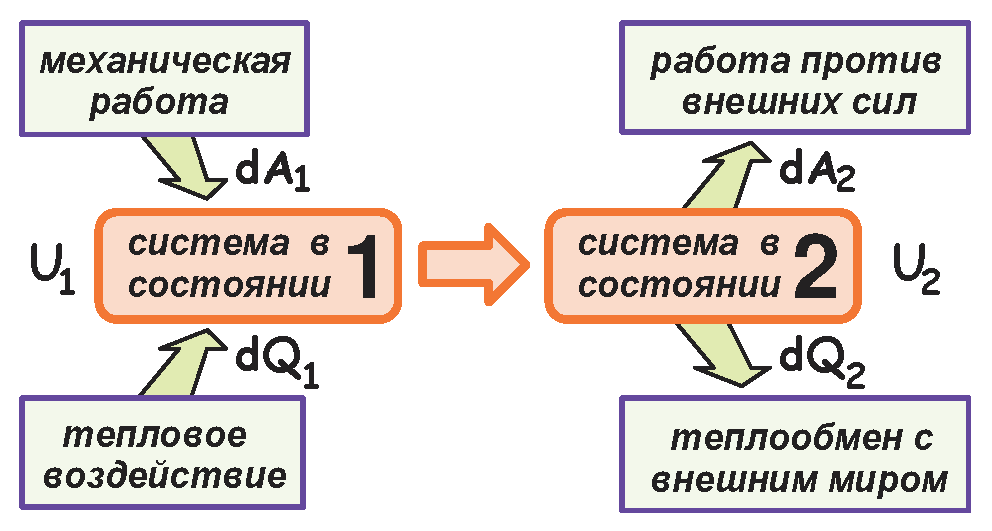
\includegraphics{GP012/GP012F02.eps}}
 \put(0,68){\makebox(0,0)[tl]{\parbox{85mm}{
 }}}
 \end{picture}\\
Внутренняя энергия системы при этом изменится на величину $dU=dA_1+dQ_1$. Поскольку не система совершила работу, а внешние силы, то $dA_1$>0. Внешний нагрев также означает $dQ_1$>0. Таким образом, оба эти воздействия УВЕЛИЧИЛИ энергию системы.

 Если затем система перейдет в состояние 2, отдав количество тепла $dQ_2$ в окружающее пространство (окружающий воздух нагрелся от контакта с цилиндром) и совершив работу $dA_2$ против внешних сил (поршень вер\-нул\-ся на прежнее место, преодолев наше сопротивление), то в итоге ее внутренняя энергия станет равной
\begin{displaymath}
U_2=U_1+dA_1+dQ_1-dA_2-dQ_2
\end{displaymath}
Здесь знаки ``--'' перед $dA_2$ и $dQ_2$ символизируют направление ПРОЧЬ ОТ СИСТЕМЫ, уменьшающее ее внутреннюю энергию.

Итак, {\bf изменение энергии системы при ее переходе из одного состояния в другое равно сумме механических экви\-ва\-лен\-тов всех внешних воздействий, ведущих к этому переходу}.

В изолированной системе внешних воздействий нет. При взаимо\-дей\-с\-т\-вии частей системы друг с другом $U$ системы сохраняется, хотя между частями энергия передается и переходит из одного вида в другой.\\
 \begin{picture}(185,60)(0,0)
 %\put(0,0){\framebox(185,60)[b]{}}
 \put(55,0){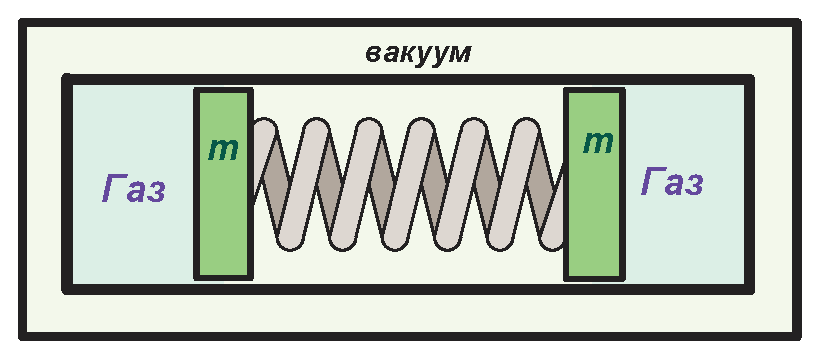
\includegraphics{GP012/GP012F03.eps}}
 \put(0,56){\makebox(0,0)[tl]{\parbox{50mm}{
\underline{Пример:}  в термосе на\-хо\-дит\-ся ци\-линдр с дву\-мя порш\-ня\-ми и пру\-жи\-ной. Пру\-жи\-на бы\-ла сжа\-та и сдер\-жи\-ва\-лась нит\-кой. Нитка лопнула!
 }}}
 \end{picture}\\
$E_p$ сжатой пружины передастся поршням и превратится в их $E_k$. Они сожмут газ, его давление возрастет и остановит поршни. При этом, вся $E_k$ поршней перейдет в $E_p$ сжатого газа. Газ толкнет остановившиеся поршни назад, и они сожмут пружину. И так далее. До бесконечности это длиться не будет: ведь даже если нет трения между поршнем и цилиндром, то есть внутреннее трение в газе! Из-за этого трения газ будет каждый раз немного нагреваться, пока вся первоначальная энергия пружины не пре\-вра\-тит\-ся в тепло. Ну, не вся, а почти вся. Ведь у {\bf нагретого} газа давление выше, и $\Rightarrow$ потенциальная энергия больше.\\

Равновесные и неравновесные системы.\\
 \begin{picture}(185,40)(0,0)
 %\put(0,0){\framebox(185,40)[b]{}}
 \put(170,0){\includegraphics{GP012/GP012F04.eps}}
 \put(0,36){\makebox(0,0)[tl]{\parbox{165mm}{
 Равновесное состояние: параметры = const без постороннего влияния.
\underline{Пример:} закрытая бутылка с вином -- это 2-фазная равновесная система жидкости и насыщенных паров. Давление и температура в разных частях бутылки -- одинаковы и не меняются со временем. соотношение $m_L/m_G$ тоже постоянно.
 }}}
 \end{picture}

Откупоренная бутылка -- неравновесна. Жидкость все время испаряется.

\underline{Другой пример:} включенный паяльник -- неравновесная система. Его жало все время подогревается спиралью, а рукоятка охлаждается воздухом.

У выключенного паяльника жало остынет, температура везде сравняется, и система станет равновесной.

Любой процесс является изменением параметров и представляет собой ряд неравновесных состояний.
Равновесный процесс состоял бы из равно\-весных состояний и должен быть бесконечно медленным. Реально такого не бывает. Но если реальный (неравновесный) процесс разложить на очень малые кусочки, то в пределах одного кусочка можно считать систему равновесной. Тогда в каждый момент можно считать, что у системы есть определенные параметры ($p, V, T$), которые меняются плавно и непрерывно,\\
 \begin{picture}(185,60)(0,0)
 %\put(0,0){\framebox(185,60)[b]{}}
 \put(0,0){\includegraphics{GP012/GP012F05.eps}}
 \put(105,0){\includegraphics{GP012/GP012F06.eps}}
 \put(40,56){\makebox(0,0)[tl]{\parbox{45mm}{
и процесс можно изобразить линией
 }}}
 \put(39,39){\vector(-1,-1){8}}
 \end{picture}\\
 Если система переходит из состояния 1 в 2, то КАКАЯ совершится РАБОТА? При малом изменении $\Delta V$ работа будет $\Delta A=p\;\Delta V$, а на всем участке --
 \begin{displaymath}
 A_{1\rightarrow2}=\int\limits_{V_1}^{V_2}p(V)\;dV
 \end{displaymath}
 При этом, конечно, должен соблюдаться ЗСЭ, поэтому изменение полной энергии системы
 \begin{displaymath}
 \Delta U_{1\rightarrow2} = U_2-U_1=Q_{1\rightarrow2}-A_{1\rightarrow2}
 \end{displaymath}
 где $Q_{1\rightarrow2}$ -- это приток тепла в систему извне.

 Если мы хотим, чтобы энергия системы не изменилась, мы должны скомпенсировать совершенную ею работу соответствующим притоком тепла.\\

 Чтобы сделать не одноразовый фокус с расширением газа, а регулярно работающую {\bf тепловую машину}, нужен {\bf циклический процесс}. Цикл (круг) -- это такой процесс, после которого система возвращается в исходное состояние (все параметры принимают первоначальные значения).\\
\noindent
  \begin{picture}(185,200)(0,0)
 %\put(0,0){\framebox(185,200)[b]{}}
 \put(0,140){\includegraphics{GP012/GP012F07.eps}}
 \put(0,70){\includegraphics{GP012/GP012F08.eps}}
 \put(0,0){\includegraphics{GP012/GP012F09.eps}}
 \put(40,200){\makebox(0,0)[tl]{\parbox{145mm}{
 Если мы пришли из состояния 1 в 2 по какой-то кривой, то работа, совершенная \underline{системой против внешних сил}, положительна:\vspace{-7mm}
 \begin{displaymath}
 \hspace{10mm}A_{1\rightarrow1}=\int\limits_{V_1}^{V_2}p^\prime(V)\;dV\;=S\prime\;>0
 \end{displaymath}
 }}}
 \put(85,160){\makebox(0,0)[tl]{\parbox{100mm}{
 По 1НТД полная энергия системы будет\vspace{-2mm}
 \begin{equation}\label{Eq.A12}
 U_2=U_1+Q_{1\rightarrow2}-A_{1\rightarrow2}\vspace*{-3mm}
 \end{equation}
 где $Q_{1\rightarrow2}$ -- приток тепла к системе.
 }}}
 \put(40,130){\makebox(0,0)[tl]{\parbox{145mm}{
 Надо теперь вернуться из 2 в 1 (можно по другому пути). Совершенная при этом работа будет отрицательной:\vspace{-2mm}
 \begin{displaymath}
 \hspace{10mm}A_{2\rightarrow1}=
  \int\limits_{V_2}^{V_1}p^{\prime\prime}(V)\;dV\;=-S^{\prime\prime}\;<0
 \end{displaymath}
 }}}
 \put(85,95){\makebox(0,0)[tl]{\parbox{100mm}{
  формально: потому, что идем налево. По смыслу: потому, что совершает работу \underline{не система}, а \underline{внешние силы}.
 }}}
 \put(20,67){\makebox(0,0)[tl]{\parbox{165mm}{
 Снова должно соблюдаться 1НТД $\Rightarrow$ полная энергия системы:\vspace{-4mm}
 \begin{equation}\label{Eq.A21}
  \hspace{15mm}U_1= U_2-Q_{2\rightarrow1}-A_{2\rightarrow1}
 \end{equation}
 }}}
 \put(185,49){\makebox(0,0)[r]{
 где $Q_{2\rightarrow1}$ -- отток тепла от системы на возвратном участке.
 }}
 \put(70,42){\makebox(0,0)[tl]{\parbox{115mm}{
 Сложив уравнения (\ref{Eq.A12}) и (\ref{Eq.A21}), получим:\vspace{-2mm}
 \begin{displaymath}
  \hspace{10mm}A\equiv A_{1\rightarrow2}+A_{2\rightarrow1}=S= Q_{1\rightarrow2}-Q_{2\rightarrow1}
 \end{displaymath}
 }}}
 \put(185,0){\makebox(0,0)[br]{\parbox{100mm}{
т.е., суммарная работа $A$, совершенная системой, численно равна площади $S$, охватываемой графиком цикла и равна
 }}}
 \end{picture}\\
разности подведенного к системе ($Q_{1\rightarrow2}$) и отведенного от нее ($Q_{2\rightarrow1}$) количества тепла.

В этом примере пути $p^\prime(V)$ и $p^{\prime\prime}(V)$ разные, причем первый из них проходит выше $\Rightarrow$ площадь $S$ и, соответственно, работа $A$, положительна. Система превратила некое тепло в работу. Это -- \fbox{\bf прямой цикл}, а изо\-бра\-жен\-ный процесс -- \fbox{\bf тепловая машина}.

Особенности прямого цикла:
\begin{itemize}
\item Чтобы закачать тепло $Q_{1\rightarrow2}$ в систему, должно присутствовать более горячее тело (нагреватель).
\item Чтобы забрать тепло $Q_{2\rightarrow1}$ от системы, должно присутствовать более холодное тело (холодильник).
\item Не все тепло $Q_{1\rightarrow2}$ превращается в работу; некоторая часть его ($Q_{2\rightarrow1}$) должна вернуться вовне. {\bf Коэффициент полезного действия} те\-п\-ло\-вой машины (к.п.д.):\vspace{-5mm}
    \begin{displaymath}
    \eta = \frac{A}{Q_{1\rightarrow2}}=\frac{Q_{1\rightarrow2}-Q_{2\rightarrow1}}{Q_{1\rightarrow2}}
    \end{displaymath}
\end{itemize}
Если возвратный путь $p^{\prime\prime}(V)$ лежит выше прямого  $p^\prime(V)$, то площадь
 $S$ и\\
 \begin{picture}(185,60)(0,0)
 %\put(0,0){\framebox(185,60)[b]{}}
 \put(0,0){\includegraphics{GP012/GP012F10.eps}}
 \put(85,59){\makebox(0,0)[tl]{\parbox{100mm}{
 работа $A$ будут отрицательными. Это значит, что система не тепло превращает в работу, а наоборот -- работу внешних сил превращает в тепло. Раз кривая $p^\prime(V)$ лежит \underline{ниже}, то происходит это расширение при более  \underline{низком} давлении и $\Rightarrow$ при более \underline{низкой} температуре. Но поскольку именно на
 }}}
 \end{picture}\\
 этом этапе система поглощает тепло, то температура нагревателя может быть ниже. Аналогично, сжатие с выделением тепла проходит при более высокой температуре $\Rightarrow$ температура холодильника, забирающего это теп\-ло у системы, может быть выше.

 Такой цикл -- это не прямой, а \fbox{\bf обратный цикл}, а процесс -- не тепловая, а \fbox{\bf холодильная машина}.\\

 Если при термодинамическом процессе теплообмена между системой и окружающим миром нет, то это -- \fbox{\bf адиабатический процесс}. В ре\-аль\-ности либо нужна супер-теплоизоляция, либо процесс должен течь настолько быстро, что теплообмен просто не успел бы произойти.
 
 %\newpage
 В адиабатическом процессе  $\Delta U + \Delta A =0$ (поскольку $\Delta Q\equiv0$).\\
 Если система совершает работу, то \hspace{15mm}$\Delta A > 0\;\;\;\Rightarrow\;\;\;\Delta U<0$.\\
 Если над системой совершают работу, то $\Delta A < 0\;\;\;\Rightarrow\;\;\;\Delta U>0$.\\
 Рассмотрим расширение 1 моля идеального газа:
 \begin{displaymath}
 \Delta A = p\;\Delta V;\hspace{10mm}
 U=\frac{i}2 kT\; N = \frac{i}2RT = C_V\;T
 \hspace{10mm}\Rightarrow\;\;\Delta U=C_V\;\Delta T
 \end{displaymath}
 тогда при \underline{адиабатическом} расширении:
 $C_V\;\Delta T + p\;\Delta V = 0.$\\
 Отсюда следует:
 \begin{itemize}
 \item при адиабатич. расширении $\Delta V>0\;\;\;\Rightarrow\;\;\;\Delta T<0$ (газ охлаждается)
 \item при адиабатическом сжатии $\Delta V<0\;\;\;\Rightarrow\;\;\;\Delta T>0$ (газ нагревается)
 \end{itemize}
 Поскольку для идеального газа $pV=RT$, то получаем диф. уравнение:
 \begin{displaymath}
  \frac{dV}{V}=-\frac{C_V}{R}\cdot\frac{dT}{T}\hspace{10mm}\texttt{или}\hspace{10mm}
  d\left(\frac{R}{C_V}\;\ln V\right)=-d\left(\ln T\right)
 \end{displaymath}
 Его решение -- это\vspace{-5mm}
 \begin{displaymath}
 T\cdot V^{\frac{R}{C_V}}={\rm const.}
 \end{displaymath}

  Вспомним, что $C_p=C_V+R$ и обозначим $C_p/C_V\equiv\gamma$. \\
  Тогда $R/C_V=\gamma-1$, и можно решение переписать как
 \begin{displaymath}
 T\cdot V^{\gamma-1}={\rm const.}\hspace{10mm}\texttt{или}\hspace{10mm}
  p\cdot V^{\gamma}={\rm const.}\hspace{10mm}(\texttt{поскольку}\hspace{5mm}
  p\;V=R\;T).
 \end{displaymath}
Эта формула Пуассона заменяет для адиабатического процесса закон Бойля-Мариотта.

 При адиабатическом переходе из состояния 1 в сост. 2
 \begin{displaymath}
 \frac{T_2}{T_1}=\left(\frac{V_1}{V_2}\right)^{\gamma-1}\hspace{10mm}
 \texttt{или}\hspace{10mm} \frac{p_2}{p_1}=\left(\frac{V_1}{V_2}\right)^{\gamma}
 \end{displaymath}
 тогда как при изотермическом переходе\vspace{-4mm}
 \begin{displaymath}
 p\;V={\rm const.}\hspace{10mm}\texttt{и}\hspace{10mm} \frac{p_2}{p_1}=\frac{V_1}{V_2}
 \end{displaymath}

Можно считать, что и {\bf адиабата}, и {\bf изотерма} -- это как бы частные случаи \fbox{\bf политропы}, причем для изотермы показатель политропы $\gamma=1$, а для адиабаты $\gamma=C_p/C_V>1$.\\
 \begin{picture}(185,65)(0,0)
 %\put(0,0){\framebox(185,65)[b]{}}
 \put(0,0){\includegraphics{GP012/GP012F11.eps}}
 \put(100,66){\makebox(0,0)[tl]{\parbox{85mm}{
Вообще-то, в природе не бывает истинных адиабат и изотерм, поскольку невозможно идеально теплоизолировать систему, как и обеспечить 100\% тепловой контакт. На самом деле, есть только политропы. Если $\gamma\simeq1$, то это близко к изотерме, а если $\gamma\simeq C_p/C_V$, то к адиабате.
 }}}
 \end{picture}\\
Кривая адиабатического процесса идет круче, чем изотермического.\\
Объяснение простое: при расширении давление уменьшается, но при этом происходит остывание газа, и из-за этого давление падает еще больше.

Пример: азот при н.у. сжимают в 5 раз адиабатически или изотермически. Разница -- ?
Решение: азот = N$_2 \Rightarrow$ i=5 степеней свободы $\Rightarrow \gamma =(i+2)/i =7/5=1.4$. \begin{itemize}
\item изотермически:
       \begin{displaymath}
       \frac{p_5}{p_1}=\frac{V_1}{V_5}\hspace{10mm}\Rightarrow\hspace{10mm}
       p_5=p_1\;\frac{V_1}{V_5}=1{\rm am}\cdot 5 = 5{\rm am}
       \end{displaymath}
\item адиабатически:
       \begin{displaymath}
       \frac{p_5}{p_1}=\left(\frac{V_1}{V_5}\right)^{1.4}\hspace{10mm}\Rightarrow\hspace{10mm}
       p_5=1{\rm am}\cdot 5^{1.4} = 9.52{\rm am}
       \end{displaymath}
       \begin{displaymath}
       \frac{T_5}{T_1}=\frac{V_1}{V_5}\hspace{10mm}\Rightarrow\hspace{10mm}
       T_5=T_1\cdot\left(\frac{V_1}{V_5}\right)^{\gamma-1}=
       300{\rm K}\cdot 5^{0.4} = 571{\rm K}=298^\circ{\rm C}
       \end{displaymath}
\item а если адиабатически сжать не в 5, а в 20 раз?
       \begin{displaymath}
       \frac{p_{20}}{p_1}=\left(\frac{V_1}{V_{20}}\right)^{1.4}\hspace{10mm}\Rightarrow\hspace{10mm}
       p_{20}=1{\rm am}\cdot 20^{1.4} = 66.3{\rm am}
       \end{displaymath}
       \begin{displaymath}
       \frac{T_{20}}{T_1}=\frac{V_1}{V_{20}}\hspace{10mm}\Rightarrow\hspace{10mm}
       T_{20}=T_1\cdot\left(\frac{V_1}{V_{20}}\right)^{\gamma-1}=
       300{\rm K}\cdot 20^{0.4} = 994{\rm K}=721^\circ{\rm C}
       \end{displaymath}
       Двигатель Дизеля! (Rudolf Diesel, 1897, Berlin)
\end{itemize}
 \begin{picture}(185,60)(0,0)
 %\put(0,0){\framebox(185,60)[b]{}}
 \put(0,0){\includegraphics{GP012/GP012F09.eps}}
 \put(80,59){\makebox(0,0)[tl]{\parbox{105mm}{
  Как мы видели, для тепловой машины с прямым циклом только часть тепла, пе\-ре\-да\-ва\-е\-мо\-го ей нагревателем, пре\-вра\-ща\-ет\-ся в работу; остальная же часть возвращается холодильнику. КПД при этом равен\vspace{-5mm}
    \begin{displaymath}
    \hspace{10mm}\eta = \frac{A}{Q_{1\rightarrow2}}=\frac{Q_{1\rightarrow2}-Q_{2\rightarrow1}}{Q_{1\rightarrow2}}
    \end{displaymath}
 }}}
 \end{picture}\\
Хотелось бы, чтоб $\eta\rightarrow1$, и тогда бы $Q_{2\rightarrow1}=0$, ничего не пришлось бы возвращать холодильнику, и он вообще стал бы не нужен! Получился бы двигатель, который просто все тепло окружающей среды превращал бы в работу ({\sl perpetuum mobile II рода}).

Но долгое время ничего не получалось. В 1824 г. Сади Карно: {\sl ``Раз\-мыш\-ления о движущей силе огня и о машинах, способных развивать эту силу''}. (Nicolas Leonard Sadi Carnot, 1796-1832, Paris). Умер от холеры, все было сожжено, больше никаких его работ не сохранилось. Главный вывод: избежать возврата $Q_{2\rightarrow1}$ невозможно.

Позднее Клаузиус и Томсон это обобщили и получили 2НТД:\\ {\bf невозможен такой периодический цикл, единственным ре\-зуль\-та\-том которого было бы получение работы за счет взятого количества тепла от одного источника.}

Другая формулировка: {\bf невозможен perpetuum mobile II рода.}\\

Тем не менее, надо к этому стремиться!  В своих ``Размышлениях'' Карно рассмотрел цикл, который теперь так и называется: \fbox{\bf цикл Карно}.
Займемся им подробнее. Цикл Карно -- это 2 изотермы и 2 адиабаты.
Идеальных изотерм и адиабат не бывает, но мы пока про это забудем. Почему вообще ИЗОТЕРМЫ? Потому что просто в это время $T_\texttt{газа}=T_\texttt{нагревателя}=$ const. Почему вообще АДИАБАТЫ? Потому что это -- противоположность изотерм (в смысле теплообмена). И вообще, если никаких специальных хитростей не выдумывать, то в природе могут быть только политропы --- все, что между изотермами и адиабатами.

 Для осуществления цикла Карно нам нужен нагреватель с темпера\-ту\-рой $T_1$, подводящий к газу тепло и заставляющий его расширяться изотермически, а также холодильник с температурой $T_3$, забирающий выделяющееся тепло при изотермическом сжатии.\\
 \begin{picture}(185,110)(0,0)
 %\put(0,0){\framebox(185,110)[b]{}}
 \put(10,0){\includegraphics{GP012/GP012F12.eps}}
 \put(100,105){\makebox(0,0)[tl]{\parbox{85mm}{
 (На адиабатических участках нет передачи тепла, поэтому там ни нагреватель, ни холодильник не нужны). }}}
 \end{picture}\\
Итак, пусть 1 моль идеального газа  -- в состоянии 1 при $p_1,V_1,T_1$.
\begin{enumerate}
\item Будем с помощью нагревателя поддерживать его при $T_1$ и дадим ему расширяться (изотермически) до состояния 2. На участке 1-2 газ получит тепло $Q_{12}$ и совершит работу $A_{12}=Q_{12}$. (Поскольку $T_1=T_2$, и газ -- идеальный, то $U=$ const.)
\item В точке 2 перестанем подогревать газ и разрешим ему расширяться адиабатически (без теплообмена) до точки 3. При этом он остынет до $T_3$ и совершит еще какую-то работу $A_{23}$.
\item Теперь начнем изотермически сжимать газ, а появляющееся тепло отводить с помощью холодильника. На пути 3-4 газ отдаст тепло $Q_{34}$ и над ним совершится работа $A_{34}=Q_{34}$. (Снова $U=$ const.)
\item В точке 4 продолжим сжимать газ, но уже без отвода тепла. Для этого потребуется еще какая-то работа $A_{41}$, и газ нагреется до $T_1$.
\end{enumerate}
В итоге, газ получит тепло\vspace{-12mm}
\begin{displaymath}
\hspace{20mm}Q_\Sigma=Q_{12}-Q_{34}\;,
\end{displaymath}
а совершенная им суммарная работа, по 1НТД равная $Q_\Sigma$,  составит
\begin{displaymath}
A_\Sigma=Q_\Sigma=A_{12}+A_{23}-A_{34}-A_{41}\;.
\end{displaymath}
Вспомнив, что  $A_{12}=Q_{12}$, а $A_{34}=Q_{34}$, с удивлением обнаружим, что
\begin{displaymath}
A_{23}=A_{41}\;,
\end{displaymath}
то есть, что в цикле Карно работа газа и работа внешних сил на адиа\-ба\-ти\-чес\-ких участках 2-3 и 4-1 компенсируют друг друга. (Это и в самом деле так; можно доказать через соответствующие интегралы).

Если же посчитать работу на изотермических участках 1-2 и 3-4, то получим:\vspace{-5mm}
\begin{displaymath}
\hspace{10mm}A_{12}=\int\limits_{V_1}^{V_2}p(V)\;dV=
\int\limits_{V_1}^{V_2}\frac{R\;T_1}{V}\;dV=
R\;T_1\left(\ln V_2-\ln V_1\right)=
R\;T_1\;\ln \frac{V_2}{V_1}\;.
\end{displaymath}
Аналогично,\vspace{-5mm}
\begin{displaymath}
-A_{34}=\int\limits_{V_3}^{V_4}p(V)\;dV=
R\;T_3\;\ln \frac{V_4}{V_3}\;.
\end{displaymath}
Но мы знаем, что при адиабатических переходах\vspace{-14mm}
\begin{displaymath}
\hspace{140mm}\frac{T_a}{T_b}=\left(\frac{V_b}{V_a}\right)^{\gamma-1}
\end{displaymath}
поэтому
\begin{displaymath}
\hspace{10mm}\left(\frac{V_4}{V_1}\right)^{\gamma-1}=
\frac{T_1=T_2}{T_4=T_3}=\left(\frac{V_3}{V_2}\right)^{\gamma-1}
\hspace{10mm}\Rightarrow\hspace{10mm}\frac{V_4}{V_1}=\frac{V_3}{V_2}
\hspace{10mm}\Rightarrow\hspace{10mm}\frac{V_4}{V_3}=\frac{V_1}{V_2}
\end{displaymath}
КПД цикла Карно равен\vspace{-5mm}
\begin{displaymath}
\hspace{40mm}\eta=\frac{A_\Sigma}{Q_{12}}=\frac{A_{12}-A_{34}}{A_{12}}=\frac{T_1-T_3}{T_1}
\end{displaymath}
и зависит только от разности температур нагревателя и холодильника!\\

 \begin{picture}(190,210)(0,0)
 %\put(0,0){\framebox(190,210)[b]{}}
 \put(0,105){\includegraphics{GP012/GP012F13.eps}}
 \put(98,105){\includegraphics{GP012/GP012F14.eps}}
 \put(0,0){\includegraphics{GP012/GP012F15.eps}}
 \put(98,0){\includegraphics{GP012/GP012F16.eps}}
 \end{picture}\\
 \begin{picture}(190,90)(0,0)
 %\put(0,0){\framebox(190,90)[b]{}}
 \put(10,0){\includegraphics{GP012/GP012F20.eps}}
 \end{picture}\\

{\bf Замечание:} цикл Карно -- идеализированный. Он -- для идеального газа; он -- для равновесных процессов $\Rightarrow$ для обратимых процессов. В жизни все сложнее, и КПД только хуже. Поэтому цикл Карно надо рас\-смат\-ри\-вать как ВЕРХНИЙ ПРЕДЕЛ для тепловых машин.\\

Любой произвольный цикл = набору $k$ циклов Карно. $\forall\; k$-го цикла $T_{1k}\leq T_{\rm max}$ и $T_{2k}\geq T_{\rm min}$, поэтому как $\forall\; k$, так и для ВСЕГО цикла вцелом
\begin{displaymath}
\eta\leq\frac{T_{\rm max}-T_{\rm min}}{T_{\rm max}}
\end{displaymath}

Для обратимого цикла Карно:
\begin{displaymath}
\eta=\frac{T_1-T_2}{T_1};\hspace{10mm}A=\eta\cdot Q_1;
\hspace{10mm}Q_2=Q_1-A=(1-\eta)\cdot Q_1=\frac{T_2}{T_1}\cdot Q_1
\end{displaymath}
откуда получаем интересное соотношение:
\begin{displaymath}
\frac{Q_2}{T_2}=\frac{Q_1}{T_1}
\end{displaymath}
Если передаваемую в каком-то процессе от тела к телу величину $S=Q/T$ назвать, например, ``приведенным количеством тепла'', то можно сказать, что в случае идеального обратимого цикла Карно приведенное количество тепла, получаемое рабочим телом (не важно -- от нагревателя или от холодильника), равно приведенному количеству тепла, отдаваемому ра\-бо\-чим телом (опять-таки, не важно, куда). Какой в этом смысл?... Если при\-ход ЧЕГО-ТО = расходу ЧЕГО-ТО, то ЭТО сохраняется.\\
Это таинственная величина -- ЭНТРОПИЯ.

Можно показать, что для НЕидеального цикла получаемое ЭТО > отдаваемого. Вообще, не только для циклов, но и для любых процессов в замкнутой системе энтропия НЕ УБЫВАЕТ (для обратимых процессов -- остается постоянной).

%\newpage
\section{Свойства ЭНТРОПИИ.}
%\underline{\bf Свойства ЭНТРОПИИ.}

\begin{itemize}
 \item Для любого (не кругового) процесса $A\rightarrow B$ энтропия системы изменяется на величину
     \begin{displaymath}
     \int\limits_A^B\frac{dQ}{T}\hspace{10mm}\Rightarrow\hspace{10mm}
     S_B=S_A+\int\limits_A^B\frac{dQ}{T}
     \end{displaymath}
     где под $Q$ понимается тепло, ПОЛУЧЕННОЕ системой.
 \item Для кругового обратимого процесса (обратимого цикла) $A\rightarrow B\rightarrow A$ энтропия системы не меняется:
     \begin{displaymath}
     \int\limits_A^B\frac{dQ}{T}+\int\limits_B^A\frac{dQ}{T}=\oint\frac{dQ}{T}=0
     \end{displaymath}
 \item Для кругового НЕобратимого процесса (если там есть хотя бы один НЕобратимый участок) энтропия системы возрастает:
     \begin{displaymath}
     \oint\frac{dQ}{T}>0
     \end{displaymath}
 \item Пример: 100 г воды охлаждаются от 15 то 0$^\circ$C. Как изменится энтропия?\\
     Решение: считая, что объем не изменился, получим $dQ=m\cdot c\cdot dT$, где $m$ -- масса, а $c$ -- удельная теплоемкость. Тогда
     \begin{displaymath}
     S_B-S_A=\int\limits_A^B\frac{dQ}{T}=\int\limits_{T_1}^{T_2}m\;c\;\frac{dT}{T}=
     m\;c\;\ln\left(\frac{T_2}{T_1}\right)=
     \end{displaymath}
     \begin{displaymath}
     =100\texttt{ г }\cdot1\texttt{ кал/г/град }\cdot\ln\frac{273}{288}=-5.34\texttt{ кал/град}
     \end{displaymath}
     минус получился потому, что энтропия уменьшилась!
  \item Для ЗАМКНУТОЙ системы она уменьшиться не может.
  \item Это все были слова об ИЗМЕНЕНИИ энтропии. А сама она чему равна? Теорема Нернста (3НТД):
      \begin{center}
      \fbox{$S(T\rightarrow0)=0$}
      \end{center}
 \end{itemize}

%\newpage
\section{Обратимые процессы:}\\
%\underline{\bf Обратимые процессы:}\\

 \begin{picture}(190,70)(0,0)
 %\put(0,0){\framebox(190,70)[b]{}}
 \put(0,0){\includegraphics{GP012/GP012F17.eps}}
 \end{picture}\\
Упругий шарик; маятник без трения; Цикл Карно; движение одной молекулы; ...\\

\section{Необратимые процессы:}\\
%\underline{\bf Необратимые процессы:}\\

{\bf Необратимым является такой процесс, обратный которому может протекать лишь как звено более сложного процесса.}\\

Для необратимого процесса характерно его {\bf направление}. \\
В {\bf положительном} направлении процесс течет ``сам собой'' \\
Работа $\longrightarrow$ тепло (когда есть трение или неупругие процессы, т.е. ВСЕГДА).\\
Перенос тепла от горячего тела к холодному.\\
Расширение газа в пустоту (убираем перегородку):\\
 \begin{picture}(190,32)(0,0)
 %\put(0,0){\framebox(190,32)[b]{}}
 \put(10,0){\includegraphics{GP012/GP012F18.eps}}
 \end{picture}\\
Чтобы загнать газ назад, нужно совершить работу по его сжатию. \\
И вообще: переход в {\bf отрицательном} направлении требует дополнительных внешних усилий, то есть, должен быть еще какой-то внешний процесс. Так, чтобы перегнать тепло от холодного к горячему (холодильная машина), нужен дополнительный положительный процесс, который совершил бы работу (она потом в виде тепла передается негревателю).

Вопрос: почему движение одной молекулы -- обратимо, а многих молекул -- нет?

Ответ: по законам статистики.\\
 \begin{picture}(190,35)(0,0)
 %\put(0,0){\framebox(190,32)[b]{}}
 \put(10,0){\includegraphics{GP012/GP012F19.eps}}
 \end{picture}\\
Пусть слева было $n$ молекул, а справа 0. После убирания перегородки все перемешалось. Какова вероятность, что слева будет $i$, а справа $j$? Если фазовые объемы и плотность вероятности слева и справа равны, то для КАЖДОЙ молекулы вероятность быть слева или справа = по 50\%. Ну, например, $n=4$. Присвоим молекулам имена: A, B, C, D -- и посмотрим, какие могут быть варианты:\\
\parbox{95mm}{
\begin{tabular}{|cccc|cccc|c|c|c|}\hline
\multicolumn{4}{|c|}{слева}&\multicolumn{4}{|c|}{справа}&i&j&$W_i$\\ \hline
A&B&C&D& & & & &4&0&1\\ \hline
A&B&C& & & & &D&3&1& \\
A&B& &D& & &C& &3&1& \\
A& &C&D& &B& & &3&1& \\
 &B&C&D&A& & & &3&1&4\\ \hline
A&B& & & & &C&D&2&2& \\
A& &C& & &B& &D&2&2& \\
 &B&C& &A& & &D&2&2& \\
A& & &D& &B&C& &2&2& \\
 &B& &D&A& &C& &2&2& \\
 & &C&D&A&B& & &2&2&6\\ \hline
A& & & & &B&C&D&1&3& \\
 &B& & &A& &C&D&1&3& \\
 & &C& &A&B& &D&1&3& \\
 & & &D& &B& & &1&3&4\\ \hline
 & & & &A&B&C&D&0&4&1\\ \hline
\end{tabular}
}\parbox{95mm}{Всего получилось 16 возможностей ($16=2^n$). Наиболее вероятен случай, когда $i=j=n/2$: 6/16=37.5\%. $W_i$ -- термодинамическая вероятность (число микросостояний). Случай, когда все 4 молекулы сами собой соберутся в левой половине, -- только ОДИН: 1/16$\simeq$6\%.
Если бы у нас было не 4 молекулы а, например, $n=10$, этот шанс еще уменьшился бы:
\begin{displaymath}
w=\frac{1}{2^{10}}=\frac{1}{1024}\simeq0.1\%
\end{displaymath}
А про МАКРО-количество и говорить нечего: при $n=10^{19}$
\begin{displaymath}
w=\frac{1}{2^{10\,000\,000\,000\,000\,000\,000}}
\end{displaymath}
}\\

Необратимый процесс -- такой, обратный которому \underline{\bf маловероятен}.
Вообще-то, кроме координат молекул надо и их скорости учитывать (вместо распределения по объему рассматривать распределение по ФАЗОВОМУ объему). Из статистики известно: система, предоставленная самой себе, стремится прийти к макросостоянию $i$, которое реализуется максимальным числом способов, т.е., к состоянию с максимальной $W_i$. Если вместо $W_i$ использовать $S\equiv k\cdot\ln W_i$, то это уже будет аддитивная величина: при разбивке системы A на 2 системы B и C, $W_A=W_B\cdot W_C$, но $S_A=S_B+S_C$! И оказывается, что определенная таким способом вел-на $S$ есть ни что иное, как ЭНТРОПИЯ! (Больцман доказал)\\

\noindent
\begin{tabular}{rcl}
Упорядоченное движение &\rule{0mm}{11mm}
 $\stackrel{\texttt{флуктуации}}{\rule[1.3mm]{30mm}{0.2mm}\!\!\rightarrow}$
 & неупорядоченное движение\\
\color{blue}
Движение тела как целого &\rule{0mm}{11mm}
 $\stackrel{\texttt{\color{blue}трение}}{\rule[1.2mm]{20mm}{0.2mm}\!\!\rightarrow}$
 & \color{blue}нагрев\\
Упорядоченное положение &\rule{0mm}{15mm}
 $\stackrel{\texttt{флуктуации}}{\rule[1.3mm]{30mm}{0.2mm}\!\!\rightarrow}$
 & неупорядоченное положение\\
\color{red}
Неоднородная смесь &\rule{0mm}{11mm}
 $\stackrel{\texttt{\color{red}диффузия}}{\rule[1.2mm]{20mm}{0.2mm}\!\!\rightarrow}$
 & \color{red}однородная смесь\\
\end{tabular}\\[5mm]

\centerline{\fbox{2НТД носит статистический характер.}}

Броуновские частицы настолько малы, что уже не подчиняются 2НТД. И вообще, ТЕРМОДИНАМИКА -- для \underline{\bf больших} статистических ансамблей.

В космических масштабах она тоже неприменима: кто сказал, что Вселенная -- это замкнутая система, что в ней должно быть равновесие, и что вообще наши модели можно рас\-про\-стра\-нять на нее? (``Тепловая смерть'' Вселенной)


\chapter{Молекулярные явления в жидкостях}
\sf\Large
%\centerline{\LARGE\bf Молекулярные явления в жидкостях}

Уравнение Ван-дер-Ваальса описывает не только реальные газы, но и жидкости. При температуре $<$ критической различие газ--жидкость ста\-но\-вит\-ся большим. Плотность жидкости и ее насыщенных паров отличается в тысячи раз. $\exists$ растянутые жидкости $\Rightarrow\exists$ прочность на разрыв.\\
 \begin{picture}(185,60)(0,0)
 %\put(0,0){\framebox(185,60)[b]{}}
 \put(0,0){\includegraphics{GP013/GP013F01.eps}}
 \put(125,55){\makebox(0,0)[tl]{\parbox{65mm}{
 В газе кинетическая энер\-гия молекул $E_k\gg$ чем энер\-гия связи $\Rightarrow$ молекулы свободно дви\-жут\-ся между столк\-но\-ве\-ни\-я\-ми, и длина свободного пробега $\lambda\gg$ размера молекул.
 }}}
 \end{picture}\\[5mm]
 Энергии не хватает, чтобы преодолеть притяжение $\Rightarrow$ жидкость занимает конечный объем.
 В жидкости расстояния между молекулами срав\-ни\-мы с их размерами $\Rightarrow$ вза\-и\-мо\-дей\-ствие $\gg$ чем в газах. Каждая молекула взаимодействует с \underline{\bf несколькими} соседними $\Rightarrow E_p=$ сумме потенциалов:\\
 \begin{picture}(185,110)(0,0)
 %\put(0,0){\framebox(185,110)[b]{}}
 \put(20,0){\includegraphics{GP013/GP013F02.eps}}
 \end{picture}
 
 %\newpage
 График для $E_p$ становится периодическим (причем учитывать надо, конечно, не ВСЕ молекулы, а только {\bf ближний порядок}:\\
 \begin{picture}(185,100)(0,0)
 %\put(0,0){\framebox(185,100)[b]{}}
 \put(20,0){\includegraphics{GP013/GP013F03.eps}}
 \end{picture}\\


В тв.теле каждый атом сидит в своей потенциальной яме и не в силах оттуда выбраться, а может там только колебаться.  У жидкости более рыхлая структура, есть свободные места -- ``дырки''.
 Поскольку $\frac12kT$ не намного < глубины ямы, то часть времени молекула ведет оседлый образ жизни, а потом из-за флуктуаций (распределение Максвелла!) переска\-ки\-ва\-ет в соседнюю ямку $\Rightarrow$ в жидкости возможна {\bf диффузия}.
Она $\ll$ чем в газе, но $\gg$ чем в тв.теле.
Только некоторые (самые быстрые) молекулы способны вырваться $\Rightarrow$ {\bf испарение}.\\
 \begin{picture}(185,50)(0,0)
 %\put(0,0){\framebox(185,50)[b]{}}
 \put(108,0){\includegraphics{GP013/GP013F04.eps}}
 \put(0,45){\makebox(0,0)[tl]{\parbox{103mm}{
{\bf Трение} в газе: перенос количества движения из слоя в слой за счет перелета молекул на длину свободного пробега. В жидкости $\exists$ еще один механизм: фононный. Шарик не только толкает правого соседа, но и тащит левого.
}}}
 \end{picture}\\
Возникает волна, которая катится по жидкости и несет импульс.\\
 \begin{picture}(185,50)(0,0)
 %\put(0,0){\framebox(185,50)[b]{}}
 \put(108,0){\includegraphics{GP013/GP013F05.eps}}
 \put(0,45){\makebox(0,0)[tl]{\parbox{103mm}{
Молекулы на {\bf поверхности}: ``соседей'' сверху НЕТ $\Rightarrow$ силы нескомпенсированы $\Rightarrow \exists$ результирующая $\neq 0$, направленная НОРМАЛЬНО к поверхности.\\ На поверхности {\em как бы} есть {\em как бы} пленка, которая хочет сжаться.
}}}
 \end{picture}\\
Явление {\bf поверхностного натяжения}. Жидкость $\rightarrow$ к сферической форме (минимальная поверхность): капли, пена, пузыри,...\\
 \begin{picture}(185,40)(0,0)
 %\put(0,0){\framebox(185,40)[b]{}}
 \put(0,0){\includegraphics{GP013/GP013F06.eps}}
 \put(110,38){\makebox(0,0)[tl]{\parbox{75mm}{
Чтобы удержать пленку от стя\-гивания, нужна сила по ка\-са\-тель\-ной к поверхности, про\-пор\-ци\-о\-наль\-ная границе:\vspace{-5mm}
\begin{displaymath}
f=\alpha\;L
\end{displaymath}
}}}
 \end{picture}\\
Коэффициент поверхностного натяжения $\alpha=f/L$ [дин/см] убывает с ростом температуры. При $T\rightarrow T_k \;\;\;\alpha\rightarrow0$. Вода (н.у.): $\alpha=73$ дин/см.\\
Если сдвинуть границу пленки $L$ на расстояние $dx$, то совершится работа $dA=f\;dx=\alpha\;L\;dx=\alpha\;dS$ (где $dS$ -- увеличение площади пленки). Эта работа идет на увеличение внутренней энергии $E$. $\Rightarrow$ еще одно определение коэф-та $\alpha$: $\alpha=dE/dS$.\\
 \begin{picture}(185,28)(0,0)
 %\put(0,0){\framebox(185,30)[b]{}}
 \put(95,0){\includegraphics{GP013/GP013F07.eps}}
 \put(0,22){\makebox(0,0)[tl]{\parbox{90mm}{
 Всплывающий пузырь не может прорвать пленку на поверхности воды $\Rightarrow$ образование пены.
}}}
 \end{picture}\\
 У мыльной воды $\alpha$ меньше, но вязкость больше, $\Rightarrow$ она медленнее вытекает из слоя между пузырем и поверхностью, и пена дольше остается.\\
  \begin{picture}(185,45)(0,0)
 %\put(0,0){\framebox(185,45)[b]{}}
 \put(0,0){\includegraphics{GP013/GP013F08.eps}}
 \put(40,40){\makebox(0,0)[tl]{\parbox{145mm}{
 Вытекающая вода образует капли, которые после отрыва принимают сферическую форму. Если давление в трубке недостаточно, то капля вообще не сможет оторваться! (Палатка пропускает воздух, а воду -- нет). Дело в соотношении диаметра трубки, кривизны капли, и т. д.
}}}
 \end{picture}\\
 \begin{picture}(185,60)(0,0)
 %\put(0,0){\framebox(185,60)[b]{}}
 \put(140,0){\includegraphics{GP013/GP013F09.eps}}
 \put(0,60){\makebox(0,0)[tl]{\parbox{135mm}{
 Рассмотрим кусочек сферической поверхности пу\-зырь\-ка с радиусом $R$. Если выделить маленькую дугу, соответствующую углу $d\varphi$, то ее длина будет $r\,d\varphi$, и
 }}}
 \put(0,37){\makebox(0,0)[tl]{\parbox{155mm}{
 сила, направленная по касательной к поверхности и $\bot$ этой дуге: $df=\alpha\,r\,d\varphi$, а ее вертикальная со\-став\-ля\-ю\-щая: $df_1=\alpha\,r\,\sin\theta\,d\varphi$. Если теперь просуммировать все силы $df_1$ от каждой из дуг, на которые разбивается граница нашего выбранного кусочка (т.е., говоря по-русски, проинтегрировать
}}}
 \end{picture}\\
  по $\varphi$, то получим суммарную силу, с которой наш кусочек поверхности площадью $\pi r^2$ давит вниз на находящуюся под ним жидкость:
  \begin{displaymath}
  f_1=\int\limits_0^{2\pi}\alpha\,r\,\sin\theta\,d\varphi=2\pi\,\alpha\,r\,\sin\theta=
  2\alpha\,\frac{\pi r^2}R
  \end{displaymath}
 а давление при этом\vspace{-6mm}
  \begin{displaymath}
  p=\frac{f_1}{S}=
  \frac{2\alpha\,\pi r^2}{R\,\pi r^2}=\frac{2\,\alpha}R
  \end{displaymath}
 \begin{picture}(185,22)(0,0)
 %\put(0,0){\framebox(185,20)[b]{}}
 \put(130,0){\includegraphics{GP013/GP013F10.eps}}
 \put(0,20){\makebox(0,0)[tl]{\parbox{125mm}{
Как видим, давление пропорционально кривизне. Если 2 пузыря соединить трубкой, то воздух потечет из маленького в большой!
}}}
 \end{picture}\\
 Если пузырь не круглый, а, например, эллиптический с радиусами кривизны $R_x$ и $R_y$, то давление в нем будет
  \begin{displaymath}
  \texttt{не }\hspace{10mm}\frac{2\,\alpha}R \;, \hspace{10mm}\texttt{ а } \hspace{10mm} p=\frac{\alpha}{R_x}+\frac{\alpha}{R_y}
  \end{displaymath}
 В частности, для цилиндрической поверхности один из радиусов = $\infty$, и давление в 2 раза меньше, чем для сферической:
  \begin{displaymath}
  p=\frac{\alpha}R \vspace*{2mm}
  \end{displaymath}

\section{Явления на границе жидкости и твердого тела} 
%\underline{\bf Явления на границе жидкости и тв.тела} \\

Два варианта:
\begin{enumerate}
 \item молекулы жидкости притягиваются друг к другу сильнее, чем к мо\-ле\-ку\-лам твердой поверхности (не смачивается)
 \item жидкость сильнее взаимодействует с твердым телом (смачивается)
\end{enumerate}
\begin{picture}(185,30)(0,0)
 %\put(0,0){\framebox(185,30)[b]{}}
 \put(85,0){\includegraphics{GP013/GP013F11.eps}}
 \put(0,30){\makebox(0,0)[tl]{\parbox{80mm}{
{\bf краевой угол $\psi$}:
\begin{enumerate}
\item $\psi>\frac\pi2$ -- не смачивается
\item $\psi<\frac\pi2$ -- смачивается
\end{enumerate}
}}}
 \end{picture}\\
\begin{picture}(185,70)(0,0)
 %\put(0,0){\framebox(185,70)[b]{}}
 \put(0,0){\includegraphics{GP013/GP013F12.eps}}
 \put(95,60){\makebox(0,0)[tl]{\parbox{90mm}{
Смачивается или нет -- зависит от веществ. Вода смачивает стекло, но не смачивает парафин. Ртуть не смачивает стекло, но смачивает железо, и т. д. Хорошо видно на капиллярах по {\bf форме мениска}. Перепад высот однозначно с этим связан (через краевой угол).
}}}
 \end{picture}\\
\begin{picture}(185,60)(0,0)
 %\put(0,0){\framebox(185,60)[b]{}}
 \put(130,0){\includegraphics{GP013/GP013F13.eps}}
 \put(0,55){\makebox(0,0)[tl]{\parbox{140mm}{
 Давление столба жидкости высотой $h$ с плотностью $\rho$ должно уравновешиваться давлением, которое создает мениск с радиусом $r$:\vspace{-10mm}
 \begin{displaymath}
  \;\;\;\;\;\;\;p=\rho g h=\frac{2\alpha}r
 \end{displaymath}
}}}
 \put(0,25){\makebox(0,0)[tl]{\parbox{125mm}{
Поскольку радиус капилляра $R$ и радиус мениска $r$ связаны через краевой угол
($R=r\cos\psi$), то высоту $h$ можно отсюда определить как
}}}
 \end{picture}\vspace{-5mm}\\
 \begin{displaymath}
  h=\frac{2\alpha}{\rho g r}=\frac{2\alpha\cos\psi}{\rho g R}
 \end{displaymath}
Если смачиваемость 100\%-ная, то $\psi=0$, и $h\rightarrow \frac{2\alpha}{\rho g R}$. Если же сма\-чи\-ва\-е\-мость нулевая, то $\psi=2\pi$, $\cos\psi=-1$, и жидкость по капилляру не поднимается, а опускается.

Если надо измерить коэф-т поверхностного натяжения $\alpha$, то можно подобрать такой материал, который бы этой жидкостью или 100\% сма\-чи\-вал\-ся, или 100\% не смачивался, и просто замерить высоту.

Капиллярность: проникновение воды в почву и другие пористые материалы; фитили; флотация.\\
\begin{picture}(185,25)(0,0)
 %\put(0,0){\framebox(185,25)[b]{}}
 \put(103,0){\includegraphics{GP013/GP013F14.eps}}
 \put(0,25){\makebox(0,0)[tl]{\parbox{98mm}{
 Если капля менее плотной жидкости растекается по более плотной, то
 $\exists$ 3 поверхностных натяжения: $\alpha_1$, $\alpha_2$ и $\alpha_{12}$
}}}
 \end{picture}\\
Силы $f_1$ и $f_{12}$ стягивают каплю, а сила $f_2$ заставляет ее растекаться. Равновесная форма капли -- когда все силы уравновешены. Это возможно при условии, что
\begin{displaymath}
 |\vec{f_2}|<|\vec{f_1}|+|\vec{f_{12}}|\hspace{10mm}\Rightarrow\hspace{10mm}
 \alpha_2<\alpha_1+\alpha_{12}
\end{displaymath}
Если же $\alpha_2$ намного больше, то капля будет растекаться бесконечно и образует мономолекулярный слой. Ленгмюр (Irving Langmuir, 1881-1957, N-Y; Нобелевская премия 1932 по химии за исследования поверхностных явлений) и Блоджетт (Katharine Blodgett, 1898-1979, N-Y). Метод при\-го\-тов\-ле\-ния мономолекулярных слоев.\\

\section{Испарение жидкостей}.\\
%\underline{\bf Испарение жидкостей}.\\

Находятся быстрые молекулы, которые преодолевают силы притяжения и, затрачивая на это преодоление некую часть энергии, вылетают из жидкости. Поскольку ее энергия при этом уменьшается, то жидкость охлаждается. Чтобы процесс шел изотермически, надо все время подводить тепло.

{\bf Удельная теплота испарения $\lambda$} -- кол-во тепла, которое надо сообщить ед-це массы жидкости, находящейся при температуре $T$, чтобы перевести ее в пар при той же температуре.   \\
$\lambda$ зависит от $T$: при $T\rightarrow T_k\;\;\lambda\rightarrow0$.\\

Если нагреть жидкость до такой $T$, при которой давление насыщенных паров = внешнему давлению, то испарение начинается не только с по\-верх\-но\-сти, но и по всему объему -- {\bf кипение}.\\

\section{Растворы}.\\
%\underline{\bf Растворы}.\\

Рассмотрим слабый раствор, когда взаимодействием растворенных молекул между собой можно пренебречь. Они образуют как бы газ (отличие от идеального газа: движению мешают молекулы растворителя).

 Средняя кинетическая энергия: $\overline{w}=\frac12\,kT$ на степень свободы.
 Сово\-куп\-ность растворенных молекул должна оказывать {\bf осмотическое} да\-в\-ле\-ние $p=\frac23\,n_0\,\overline{w}$, и для них должно соблюдаться уравнение Менделеева-Кла\-пейрона:
 \begin{displaymath}
  pV=\frac m\mu RT
 \end{displaymath}
\begin{picture}(185,75)(0,0)
 %\put(0,0){\framebox(185,75)[b]{}}
 \put(155,0){\includegraphics{GP013/GP013F15.eps}}
 \put(0,75){\makebox(0,0)[tl]{\parbox{150mm}{
 Если в растворе установить полупроницаемую мембрану (например, пропускающую воду, но не пропускающую растворенный в ней сахар), то сверху будет только давление воды, а снизу -- воды + сахара. Поэтому наверх будет проникать молекул воды больше, чем вниз, до тех пор, пока давление не уравновесится. Если равновесие наступило $\Rightarrow$ осмотическое (парциальное) давление сахара = дополнительному давлению столба воды $p=\rho\,g\,h$.
 Если обозначить концентрацию раствора как $C\equiv m/V$, то получаем \fbox{формулу Вант-Гоффа}:
}}}
 \end{picture}\\[-5mm]
 \begin{displaymath}
  p=\frac{C}\mu\, R\,T
 \end{displaymath}

 (Jacobus Henricus van 't Hoff, 1852-1911, Rotterdam; 1901 г.: Нобелевская премия по химии)

 При измерении осмотического давления для растворов разных веществ было найдено, что во многих случаях результаты согласуются с формулой Вант-Гоффа, но не всегда. Для растворов неорганических солей осмоти\-чес\-кое давление существенно БОЛЬШЕ. Причина: при растворении они диссоциируют на части, число частиц на единицу объема растворителя возрастает, а поскольку  $p=\frac23\,n_0\,\overline{w}$, то и осмотическое давление тоже возрастает.

 Те растворы, что подчиняются формуле Вант-Гоффа, -- не проводят эл.ток, а те, где $\exists$ диссоциация, -- проводят! Вывод: диссоциация идет не на АТОМЫ, а на ИОНЫ.


\chapter{Колебания и волны}
\input{GP014/GP014_section.tex}

\chapter{Электростатика}
\input{GP015/GP015_section.tex}

\chapter{Классическая электронная теория (КЭТ)}
\input{GP017/GP017_section.tex}

\chapter{Электромагнитный масс-сепаратор}
\input{GP019/GP019_section.tex}

\chapter{Атомная физика}


%\vspace*{-20mm}
% \centerline{\underline{\Large\bf Атомная физика}}\vspace{5mm}

\centerline{\large\bf Проблема: у света $\exists$ корпускулярные свойства
 (а не только волновые!)}
\begin{itemize}
\item Если считать суммарную мощность излучения абсолютно черного тела по классической электродинамике (Рэлей \& Джинс), то получается {\bf абсурдный} результат ($W x\rightarrow\infty$). Но все становится разумным, если верна непонятная гипотеза {\bf Макса Планка} о том, что излучение не непрерывно, а возможно лишь порциями $\varepsilon=h\nu$, где $h=6.624\cdot10^{-27}$ эрг (постоянная Планка), а $\nu$ -частота излучения.
\item В рентгеновском спектре $\exists$ {\bf левая граница} ($\lambda\geq\lambda_{min}$), зависящая от напряжения питания рентгеновской трубки U: $\lambda_{\rm min}$[{\AA}]=12350/U[V]. То есть, вроде как и в самом деле один электрон с $E=eU$ не может породить фотон с $h\nu=\varepsilon>E$.
\item {\bf Фотоэффект}: ток не зависит от напряжения ($\exists$ насыщение), но пропорционален ин\-тен\-сив\-но\-с\-ти облучения светом; тока нет совсем, если $\lambda\geq\lambda_{\rm min}$ (то есть, если энергия одного фотона < работы выхода электрона из облучаемого металла). При уменьшении $\lambda$ энегрия выбитых электронов растет линейно с частотой света. Кроме того, фотоэлектроны появляются {\bf сразу} после начала облучения (даже если свет ОЧЕНЬ слабый) --  то есть, нет ``накопления'' энергии слабой волны до порогового значения.
\end{itemize}
{\bf Альберт Эйншнейн}: не только излучение, но и поглощение света идет {\bf КВАНТАМИ}.
Вывод: свет -- это ФОТОНЫ (=кванты электромагнитного излучения). Свойства -?

\begin{itemize}
\item Энергия фотона: $\varepsilon=h\nu$\\
 \begin{tabular}{lrcc}
 ИК:  & $\lambda=10\mu m$ & $\varepsilon=2\cdot 10^{-13}$ эрг & $\simeq 0.1$ эВ\\
 видимый свет:  &$\lambda$=5000{\AA} & $\varepsilon=4\cdot10^{-12}$ эрг & $\simeq 2.5$ эВ\\
 X-лучи:  &$\lambda$=0.1 {\AA} & $\varepsilon=2\cdot10^{-7}$ эрг & $\simeq 70$ кэВ\\
 \end{tabular}\\
 Корпускулярные св-ва проявляются сильнее при больших энергиях (малых $\lambda$)
\item Масса фотона =0 (т.к. фотон {\sl по определению} движется со скоростью света, а энергия не $\infty$, то его масса по законам релятивистской механики просто обязана быть $\equiv$ 0).
\item Количество движения (импульс) фотона связан с его энергией:
\begin{displaymath}
E^2=\left(mc^2\right)^2+(pc)^2\hspace{20mm}(m=0)\Rightarrow\hspace{10mm}E=pc\hspace{10mm}\Rightarrow\hspace{10mm}
p=\frac{h\nu}c
\end{displaymath}
И действительно, известно ``световое давление''!
\item {\bf Артур Комптон} (1923): рассеяние Х-лучей. Среди рассеянных $\exists$ лучи не только с $\lambda=\lambda_0$, но и с $\lambda>\lambda_0$!!! \\
    Объяснение: до рассеяния был фотон с энергией $h\nu_1$ и импульсом $\vec{p}_\gamma$ + покоящийся $e^-$. После рассеяния $e^-$ приобрел отдачу (энергию $E_e$ и импульс $\vec{p}_e$), а фотон ЭТО ЖЕ потерял: $h\nu_2 = h\nu_1 - E_e$, \hspace{10mm} $\vec{p}_2=\vec{p}_1-\vec{p}_e$. Если все аккуратно посчитать, то можно получить известную формулу:
\begin{displaymath}
E_1-E_2=\frac{E_1E_2}{mc^2}\;(1-\cos\varphi)\hspace{20mm}\texttt{или}\hspace{20mm}
 \lambda_2-\lambda_1=\frac{hc}{mc^2}\;(1-\cos\varphi)
\end{displaymath}
где $\varphi$ -- угол рассеяния фотона.
\end{itemize}
Но и волновые свойства света никто не отменял (интерференция, дифракция, поляризация, отражение, преломление)...\\
Накопилось много фактов, толкающих к созданию новой (не классической) физики, которая бы все это как-то объясняла.\\

%\newpage
\section{Проблемы со строением атома}
%\centerline{\Large\bf Проблемы со строением атома.}

\begin{picture}(190,50)(0,0)
\put(50,0){\includegraphics{GP028/GP028F01.eps}}
 \put( 50,45){\makebox(0,0)[lt]{\bf Модель Томсона}}
 \put(90,45){\makebox(0,0)[lt]{\bf Модель Резерфорда}}
 \put(0,38){\makebox(0,0)[lt]{\parbox{52mm}{
 Атом -- это равномерно (или почти равномерно) положительно заряженный шарик, и в нем мечутся точечные отрицательные электроны).
 }}}
 \put(180,38){\makebox(0,0)[rt]{\parbox{57mm}{
 Атом -- это положительно заряженное точечное мас\-сив\-ное ядро, и вокруг него (как планеты вокруг Солнца) летают точечные отрицательные электроны).
 }}}
\end{picture}\\[5mm]
Первая модель: почему заряженный рыхлый шарик не разваливается? Если он не рыхлый -- то как электрон через него проникает? \\
Вторая модель лучше. Но непонятно: почему движущийся электрон не излучает и почему он не падает на ядро?\\
Опыт Резерфорда по рассеянию $\alpha$-частиц: если бы шарик был рыхлым, то не было бы рассеяния на большие углы (а оно бывает). Вывод: ядро есть! Но почему же нет излучения?...\\[10mm]
%\vspace*{5mm}

\section{Проблемы с оптическими спектрами}
%\centerline{\Large\bf Проблемы с оптическими спектрами.}\\[3mm]

{\bf Бальмер} (Базель, 1885): в линейчатых спектрах испускания $\exists$ какая-то странная закономерность.\\
\begin{picture}(190,30)(0,0)
\put(10,0){\includegraphics{GP028/GP028F02.eps}}
\end{picture}\\[5mm]
\begin{displaymath}
\lambda_n=\lambda_0\cdot\frac{n^2}{n^2-4}
\end{displaymath}
где $n$ -- некоторое целое число: $n$=3, 4, 5, ...

В спектроскопии традиционно вместо обычной частоты принято использовать волновое число $\nu$ (сколько $\lambda$ уместится в 1 см):
\begin{displaymath}
\nu\equiv\frac{1 \texttt{см}}\lambda \hspace{10mm}[\nu]={cm}^{-1}.
\end{displaymath}
Так вот, у Бальмера получилось, что для многих атомов $\nu=A-R/n^2$.

Позднее {\bf Ридберг} (Лунд, Швеция, 1888) определил, что $A=R/4$ (выполняется очень точно!), и тогда можно сказать, что
\begin{displaymath}
 \nu =R\cdot\left(\frac1{2^2}-\frac1{n^2}\right)\hspace{20mm}R=109737.316\;\; {cm}^{-1}
\end{displaymath}
(потом эту константу $R$ назвали постоянной Ридберга).

Получалось, что есть какие-то ТЕРМЫ (наподобие энергетических уровней), и излучение -- это комбинация РАЗНОСТЕЙ между термами. Для них даже придумали названия: 1S, 2P, 3P, 4D, и т.д.

В это время {\bf Нильс Бор} (Копенгаген, 1913) как раз думал об устройстве атома. {\em ``Как только я увидел формулу Бальмера, весь вопрос стал мне немедленно ясен.'' }

\section{Атом, который построил Бор}
%{\Large \bf Атом, который построил Бор}

Есть {\bf дискретные стационарные} состояния атома. Находясь в них, атом ничего не излучает. Излучение возникает (или поглощается) только при переходе между состояниями. Что это за состояния? Бор: стационарными являются лишь те, для которых угловой момент количества движения ($\mathcal{L}=pr=\mathcal{I}\omega=m\cdot v\cdot r$)
кратен целому числу:
\begin{displaymath}
\mathcal{L}=n\cdot\hbar=n\cdot\frac{h}{2\pi}\hspace{20mm}\left(\hbar=\frac{h}{2\pi}\right)
\end{displaymath}
Если считать, что электрон крутится по круговой орбите с радиусом $r$ и удерживается на ней кулоновской силой, то:
\begin{displaymath}
\texttt{(центростремительная сила:) }
\frac{mv^2}r =\frac{Ze^2}{r^2}
\texttt{ (- кулоновскаяая сила)}
\end{displaymath}
учтем, что по Бору $mvr=n\hbar$,  избавимся от $v$ и затем найдем $r$:
\begin{displaymath}
v=\frac{n\hbar}{mr}\hspace{20mm} \frac{mn^2\hbar^2}{m^2r} =Ze^2\hspace{20mm}r=\frac{n^2\hbar^2}{Zme^2}
\end{displaymath}
Если теперь вычислить первый боровский радиус $a_0$ (то есть, положить $Z$=1 и $n$=1), то получим нечто очень похожее на правду:
\begin{displaymath}
a_0=\frac{\hbar^2}{me^2}=0.529\;\;{\texttt{\AA}}
\end{displaymath}
Полная энергия =
\begin{displaymath}
W_p+W_k=-\frac{Ze^2}{r}+\frac{mv^2}2=-\frac{Ze^2}{r}+\frac{Ze^2}{2r}=-\frac{Ze^2}{2r}=
-\frac{Ze^2\;Zme^2}{2\;n^2\hbar^2}=-\frac{mZ^2e^4}{2\hbar^2n^2}
\end{displaymath}
При переходе с $n_1$ на $n_2$ частота будет
\begin{displaymath}
\nu=\frac{\varepsilon}{h}=\frac{W_1-W_2}{h}=\frac{mZ^2e^4}{4\pi\hbar^3}\cdot\left(\frac1{n_1^2}-\frac1{n_2^2}\right)
\end{displaymath}
и, следовательно, в серии Бальмера были переходы с $n_1$=3,4,5,.. на $n_2$=2. Значит, должны еще где-то быть и другие серии, например: $n_1$=2,3,4,5,.. на $n_2$=1.  После такого предсказания Бора Лайман действительно нашел эту серию (просто она в УФ-диапазоне была, поэтому ее раньше не заметили).

Если еще учесть, что не только электрон движется, но и ядро, то получается совсем хорошо: даже видна разница между протием и дейтерием (в 4-ом знаке отличие). Короче, после Бора в оптике наступила эйфория. Непонятно только было, ПОЧЕМУ так все хитро устроено? \\[5mm]
{\bf Луи де Бройль} (Louis-Victor-Pierre-Raymond, 7\`{e}me duc de Broglie, Дьепп, 1924):  Может, не только у света есть корпускулярные свойства, но и у всех частиц -- волновые?...  Если мы фотону с длиной волны $\lambda$ (или частотой $\nu$) сопоставляем энергию $\varepsilon=h\nu$ и импульс $p=h\nu/c=h/\lambda$, то почему бы {\em``нормальной''} частице, имеющей энергию $\varepsilon$ и импульс $p=mv$ не сопоставить какую-то волну с длиной $\lambda=h/p$? (Поскольку $\varepsilon=h\nu=h/T=hc/\lambda$, а $p=\varepsilon/c=h/\lambda$)

Когда через 3 года экспериментально была обнаружена дифракция электронов на кристалле, за эту дерзкую мысль Луи де Бройлю была вручена Нобелевская премия.

Например, при $E_e=1$ кэВ дебройлевская длина волны электрона $\lambda=h/mv=h/\sqrt{2mE}\simeq0.4${\AA}, то есть, схожа с рентгеном. Поскольку электроны легко можно разогнать до МэВ, то $\lambda$ будет еще короче, и, следовательно, можно сделать электронный микроскоп, способный различать совсем малые объекты (в 1000 раз меньше, чем оптический).

Каков физический смысл такой как бы волны? Чтобы не путать с другими (настоящими) волнами, ее называют волновой функцией, зависящей от координат и времени: $\Psi(x,y,z,t)$. Если поле, в котором частица движется, стационарно (а мы до других случаев в этом курсе не дойдем), то можно ее представить в виде двух сомножителей:
\begin{displaymath}
\Psi(x,y,z,t)=f(t)\;\psi(x,y,z)
\end{displaymath}
Если в пространстве, где находится наша частица, выделить объемчик $dV$, настолько маленький, чтобы можно было считать $\psi(x,y,z)$=const в его пределах, то тогда вероятность обнаружить частицу именно в этом объемчике будет равна
\begin{displaymath}
dW=|\psi(x,y,z)|^2\cdot dV
\end{displaymath}
Ну вот и обнаружился физический смысл ({\bf Макс Борн}, Г\"{e}ттинген):  {\bf квадрат волновой функции -- это плотность вероятности нахождения частицы в данной точке}:
\begin{displaymath}
|\psi(x,y,z)|^2=\frac{dW}{dV}.
\end{displaymath}
Поскольку ну где-то она же просто обязана быть, то получаем и условие нормировки:
\begin{displaymath}
\int\limits_V|\psi(x,y,z)|^2\;dV\;=1.
\end{displaymath}
Волновые функции (как и обычные волны) могут интерферировать, и тогда где-то могут образоваться максимумы, а где-то -- минимумы.

Итак, каждая частица (и фотон в том числе) -- это именно {\bf частица}, а не волна. Как волну же ее можно рассматривать в том смысле, что куда она попадет -- никто не знает. Можно подсчитать только ее волновую функцию в разных точках пространства и в разные моменты времени (способ расчета -- такой же, как если бы это и вправду была волна). Полученный результат (точнее, его квадрат) дает нам вероятность того, что частица окажется именно там и именно тогда.

Если мы получаем интерференционную картину, то это не значит, что один фотон (или один электрон -- неважно) ``размазывается'' по экрану! Нет. один фотон попадает в одну точку. Другое дело, что мы не знаем -- в какую. Можем только сказать, что вот сюда он попадет с большей вероятностью, а завернет за угол -- с меньшей (но, заметьте: не с нулевой!).\\[5mm]

{\bf Вернер Гейзенберг} (Мюнхен, 1930): соотношение неопределенностей: $\Delta x\;\Delta p\geq \hbar$ или $\Delta t\;\Delta E\geq \hbar$.

Некоторые полагают, что в процессе измерения мы влияем на частицу и поэтому не можем определить сразу и координату, и скорость. Но дело не в этом.

Пример: если мы хотим измерить скорость, то мы не можем сделать это мгновенно -- мы должны отмерить какое-то НЕНУЛЕВОЕ расстояние и засечь, за какое время частица это расстояние пройдет. Так {\bf где же} мы измерили скорость -- в начале нашего ``мерного отрезка'' или в его конце? Вот вам и неопределенность.

Другой пример: хотим измерить энергию фотона, то есть, его частоту. Но чтобы измерить ЧАСТОТУ, надо в течение какого-то времени (хотя бы одного периода) понаблюдать за величиной напряженности (или что там в этой волне колеблется). То есть, опять-таки, для измерения $E$ с точностью $\Delta E$ нужно время $\Delta t$. Причем, если $E$ хочется узнать поточнее ($\Delta E\rightarrow0$) , то одного периода будет для измерения мало, и $\Delta t$ возрастет.

Если есть какое-то возбужденное состояние системы, и она там находится недолго  ($\Delta t\rightarrow0$), то энергию возбуждения точно измерить не представляется возможным (в этих случаях вместо времени жизни зачастую приводят ширину уровня). Отсюда проистекает возможность оперирования с виртуальными частицами: на очень короткое время можно забыть о сохранении энергии и считать, что новые частицы могут рождаться пачками, а потом очень быстро исчезать.\\[5mm]

Еще один постулат квантовой механики -- это аналог второго закона Ньютона (предложен {\bf Эрвином Шр\"{e}дингером}, Вена):
\begin{displaymath}
-\frac{\hbar^2}{2m}\left(\frac{\partial^2\Psi}{\partial x^2}+\frac{\partial^2\Psi}{\partial y^2}+\frac{\partial^2\Psi}{\partial z^2}\right)+E_p(x,y,z)\Psi=i\hbar\frac{\partial\Psi}{\partial t}
\end{displaymath}
Все это вы будете решать, проходя курс квантовой физики в 4 семестре. Если рассмотреть самый простой случай (частица находится в одномерной прямоугольной бесконечно глубокой потенциальной яме), то от уравнения остается всего лишь
\begin{displaymath}
-\frac{\hbar^2}{2m}\cdot\frac{\partial^2\Psi}{\partial x^2}=i\hbar\frac{\partial\Psi}{\partial t}
\end{displaymath}
Если еще и во времени ничего не меняется, то все еще больше упрощается и сводится к
\begin{displaymath}
-\frac{\partial^2\psi}{\partial x^2}=\omega^2\psi\hspace{20mm}\texttt{где}\hspace{10mm}
 \omega^2=\frac{2mE}{\hbar^2}
\end{displaymath}
Решение этого уравнения -- гармоническая функция $\psi=\psi_0\;\cos(\omega x+\varphi_0)$. Подставляя сюда граничные условия ($\psi(x=0)=0$ и $\psi(x=L)=0$, где $L$ -- ширина ямы), получим:
\begin{displaymath}
\psi_0\;\cos(\omega L+\frac{\pi}2)=0
\end{displaymath}
откуда следует, что $\omega =n\pi/L$, где $n$ - целое число. Энергия $E=\hbar^2\omega^2/2m=h^2n^2/8mL^2$. Как видим, получился набор дискретных решений ($n=1,2,..$) с разной энергией и разной плотностью вероятности в пределах ямы. Если решать не одномерную, а сферическую задачу с атомом водорода, то получится все так же, но там вместо переменных $x, y, z$ будут сферические координаты:
\begin{displaymath}
\psi(r,\theta,\varphi)=f_1(r)\;f_2(\theta)\;f_3(\varphi).
\end{displaymath}
При решении снова возникают гармонические волны, из которых получается набор квантовых чисел:
\begin{enumerate}
\item главное число $n=1,2,3,4,..\infty$
\item орбитальное число $l=0,1,2,3,.., n-1$; при этом величина орбитального момента с этим числом связана так: $\mathcal{L}=\hbar\sqrt{l(l+1)}$
\item магнитное квантовое число $m_l=0,\pm1,\pm2,\pm3,.., \pm l$; оно характеризует проекцию орбитального момента на произвольное выделенное направление (например, на направление внешнего поля, или на ось пучка);
\item спиновое квантовое число $m_s=\pm1/2$; как и число $m_l$, оно характеризует проекцию углового момента, только не орбитального, а собственного момента электрона (его спина), который равен 1/2.
\end{enumerate}
Чтобы не нарушать сложившихся в спектроскопии традиций, решено было сохранить ранее принятые обозначения термов:\\
1S = (n=1 l=0 $m_l=0 \;\;m_s=\pm1/2$)\\
2S = (n=2 l=0 $m_l=0 \;\;m_s=\pm1/2$)\\
2P = (n=2 l=1 $m_l=0,\pm1 \;\;m_s=\pm1/2$)\\
3S = (n=3 l=0 $m_l=0 \;\;m_s=\pm1/2$)\\
3P = (n=3 l=1 $m_l=0,\pm1 \;\;m_s=\pm1/2$)\\
3D = (n=3 l=2 $m_l=0,\pm1,\pm2 \;\;m_s=\pm1/2$)\\
4S = (n=4 l=0 $m_l=0 \;\;m_s=\pm1/2$)\\
4P = (n=4 l=1 $m_l=0,\pm1 \;\;m_s=\pm1/2$)\\
4D = (n=4 l=2 $m_l=0,\pm1,\pm2 \;\;m_s=\pm1/2$)\\
4F = (n=4 l=3 $m_l=0,\pm1,\pm2,\pm3 \;\;m_s=\pm1/2$)\\
и т. д.

Спиновый и орбитальный моменты могут взаимодействовать с внешним полем либо каждый сам по себе, либо сперва объединившись в один полный момент (спин-орбитальное взаимодействие) -- в этом случае вместо $m_l$ и $m_s$ надо использовать новые квантовые числа: полный момент $j=l\pm s$ и его проекцию $m_j=-j\ldots+j$.

Вот теперь, после появления квантовой механики в 1924 г. (Гейзенберг, Шредингер, Борн) атомная модель Нильса Бора обрела настоящий смысл. Она смогла наконец-то объяснить не только простейший атом водорода, но и много-электронные атомы. Для этого пришлось учесть: 1) что энергия зависит не только от $n$, но и от $l$ и $j$, а при наличии внешних полей -- еще и от всех проекций $m$; 2) принцип Паули, запрещающий существование более одной частицы со всеми одинаковыми квантовыми числами.



\backmatter
% Ссылки, глоссарий, индекс и т.д., если необходимо

\end{document}
